\mode*
\part{Memory Management}

\lecture[mm]{mm}{mm}

\section{Background}

\begin{frame}{Memory Management}
  \begin{description}
  \item[In a perfect world] Memory is \emph{large, fast, non-volatile}
  \end{description}
  \begin{block}{In real world ...}
    \begin{center}
      \mode<beamer>{ 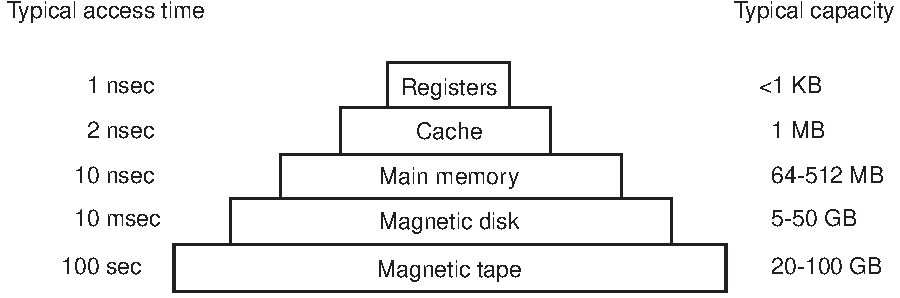
\includegraphics[width=\textwidth]{mos-figs-1-7} }%
      \mode<article>{ 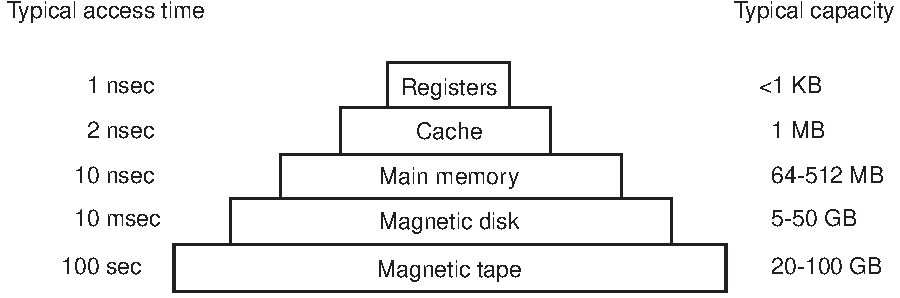
\includegraphics[width=.6\textwidth]{mos-figs-1-7} }
    \end{center}
  \end{block}
  \begin{itemize}
  \item[] Memory manager handles the memory hierarchy.
  \end{itemize}
\end{frame}

\begin{frame}{Basic Memory Management}{Real Mode}
  \begin{block}{In the old days ... }
    \begin{itemize}
    \item Every program simply saw the physical memory
    \item mono-programming without swapping or paging
    \end{itemize}
    \begin{center}
      \mode<beamer>{ \includegraphics[width=\textwidth]{mm-realmode} }%
      \mode<article>{ \includegraphics[width=.5\textwidth]{mm-realmode} }
    \end{center}
  \end{block}
\end{frame}

\begin{frame}{Basic Memory Management}{Relocation Problem}
  \begin{center}
    \mode<beamer>{ \includegraphics[width=.7\textwidth]{mm-relocation} }%
    \mode<article>{ \includegraphics[width=.5\textwidth]{mm-relocation} }
  \end{center}
\end{frame}

\begin{enumerate}
\item[(a)] only one program in memory
\item[(b)] only another program in memory
\item[(c)] both in memory
\end{enumerate}

\begin{frame}{Memory Protection}{Protected mode}
  We need
  \begin{itemize}
  \item Protect the OS from access by user programs
  \item Protect user programs from one another
  \end{itemize}
  \begin{description}
  \item[Protected mode] is an operational mode of x86-compatible CPU.
    \begin{itemize}
    \item The purpose is to protect everyone else (including the OS) from your program.
    \end{itemize}
  \end{description}
\end{frame}

\begin{frame}{Memory Protection}{Logical Address Space}
  \begin{description}
  \item[Base register] holds the smallest legal physical memory address
  \item[Limit register] contains the size of the range
  \end{description}
  \begin{varwidth}{.48\textwidth}
    \begin{center}
      \mode<beamer>{
        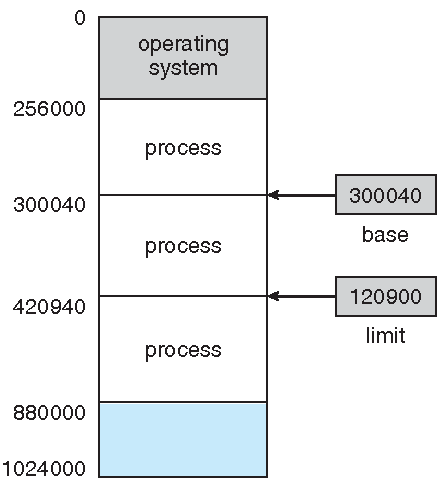
\includegraphics[width=\textwidth]{osc-8-5}
      } \mode<article>{
        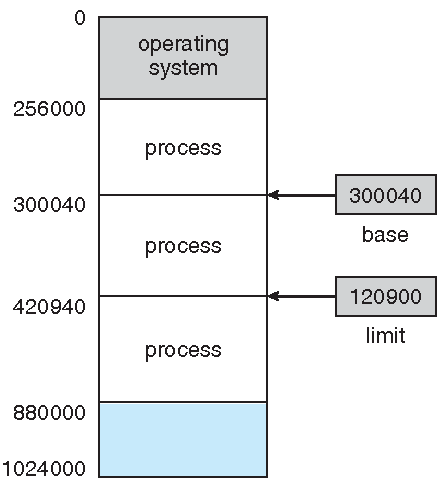
\includegraphics[width=.7\textwidth]{osc-8-5}
      }
    \end{center}
  \end{varwidth}\hfill
  \begin{varwidth}{.45\textwidth}
    A pair of \texttt{base} and \texttt{limit} registers define the logical address space
    \begin{center}
      \cfbox{violet}{\texttt{JMP 28}}
    \end{center}
    \begin{center}
      {\rotatebox{270}{\huge \Symbol{➠}}}
    \end{center}
    \begin{center}
      \cfbox{violet}{\texttt{JMP 300068}}
    \end{center}
  \end{varwidth}
\end{frame}

\begin{frame}{Memory Protection}{Base and limit registers}
  \begin{center}
    \mode<beamer>{
      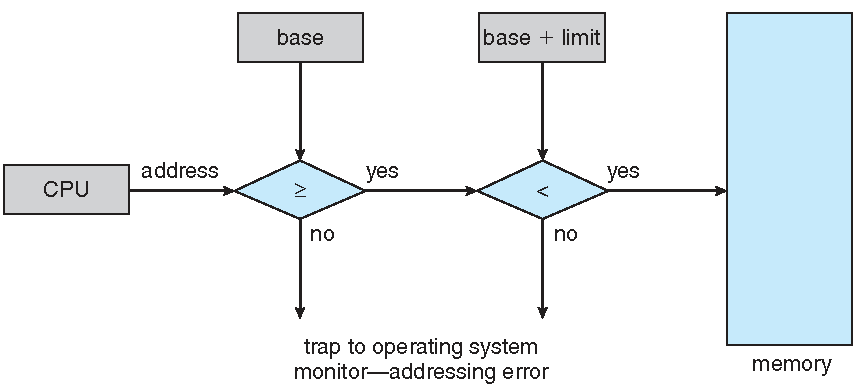
\includegraphics[width=\textwidth]{mm-protection}
    }
    \mode<article>{
      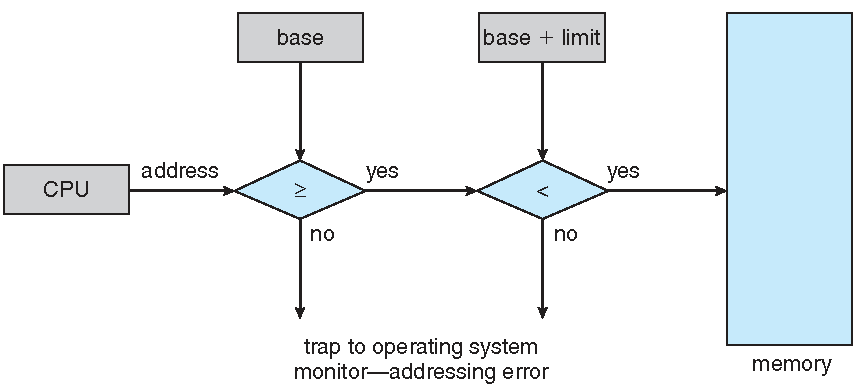
\includegraphics[width=.7\textwidth]{mm-protection}
    }
  \end{center}
\end{frame}

\begin{frame}{UNIX View of a Process' Memory}
  \begin{varwidth}{.48\textwidth}
    \begin{center}
      \mode<beamer>{
        \includegraphics[width=\textwidth]{mm-process}
      } \mode<article>{
        \includegraphics[width=.7\textwidth]{mm-process}
      }
    \end{center}
  \end{varwidth}\hfill
  \begin{varwidth}{.48\textwidth}
    \begin{itemize}
    \item[text:] program code
    \item[data:] initialized global and static data
    \item[bss:] uninitialized global and static data
    \item[heap:] dynamically allocated with \texttt{malloc, new}
    \item[stack:] local variables
    \end{itemize}
  \end{varwidth}
\end{frame}

\begin{frame}{Stack vs. Heap}
  \begin{center}
    \begin{tabular}{ll}\hline
      \thead{Stack}           &\thead{Heap}\\\hline
      compile-time allocation &run-time allocation\\
      auto clean-up           &you clean-up\\
      inflexible              &flexible\\
      smaller                 &bigger\\
      quicker                 &slower\\\hline
    \end{tabular}
  \end{center}
  \begin{block}{How large is the ...}
    \begin{description}
    \item[stack:] \texttt{ulimit -s}
    \item[heap:] could be as large as your virtual memory
    \item[text|data|bss:] \texttt{size a.out}
    \end{description}
  \end{block}
\end{frame}

\begin{frame}{Multi-step Processing of a User Program}{When is space
    allocated?}
  \begin{minipage}{.4\textwidth}
    \begin{center}
      \mode<beamer>{ \includegraphics[width=\textwidth]{tool-chain} }%osc-8-7
      \mode<article>{ \includegraphics[width=.9\textwidth]{tool-chain} }
    \end{center}
    \label{reg}
  \end{minipage}
  \begin{minipage}{.55\textwidth}
    \begin{small}
      \begin{description}
      \item[Static:] before program start running
        \begin{itemize}
        \item Compile time
        \item Load time
        \end{itemize}
      \item[Dynamic:] as program runs
        \begin{itemize}
        \item Execution time
        \end{itemize}
      \end{description}
    \end{small}
  \end{minipage}
\end{frame}

\begin{description}
\item[Compiler] The name "compiler" is primarily used for programs that translate source
  code from a high-level programming language to a lower level language (e.g., assembly
  language or machine code)\citetitle{wiki:compiler}.
\item[Assembler] An assembler creates object code by translating assembly instruction
  mnemonics into opcodes, and by resolving symbolic names for memory locations and other
  entities\citetitle{wiki:assembler}.
\item[Linker] Computer programs typically comprise several parts or modules; all these
  parts/modules need not be contained within a single object file, and in such case refer
  to each other by means of symbols\citetitle{wiki:linker}.

  When a program comprises multiple object files, the linker combines these files into a
  unified executable program, resolving the symbols as it goes along.

  Linkers can take objects from a collection called a library. Some linkers do not include
  the whole library in the output; they only include its symbols that are referenced from
  other object files or libraries. Libraries exist for diverse purposes, and one or more
  system libraries are usually linked in by default.

  The linker also takes care of arranging the objects in a program's address space. This
  may involve relocating code that assumes a specific base address to another base. Since
  a compiler seldom knows where an object will reside, it often assumes a fixed base
  location (for example,zero).
\item[Loader] An assembler creates object code by translating assembly instruction
  mnemonics into opcodes, and by resolving symbolic names for memory locations and other
  entities. ... Loading a program involves reading the contents of executable file, the
  file containing the program text, into memory, and then carrying out other required
  preparatory tasks to prepare the executable for running. Once loading is complete, the
  operating system starts the program by passing control to the loaded program
  code\citetitle{wiki:loader}
\item[Dynamic linker] A dynamic linker is the part of an operating system (OS) that loads
  (copies from persistent storage to RAM) and links (fills jump tables and relocates
  pointers) the shared libraries needed by an executable at run time, that is, when it is
  executed. The specific operating system and executable format determine how the dynamic
  linker functions and how it is implemented. Linking is often referred to as a process
  that is performed at compile time of the executable while a dynamic linker is in
  actuality a special loader that loads external shared libraries into a running process
  and then binds those shared libraries dynamically to the running process. The specifics
  of how a dynamic linker functions is operating-system
  dependent\citetitle{wiki:dynamic-linker}
\end{description}

Linkers and Loaders allow programs to be built from modules rather than as one big
monolith.

See also:
\begin{itemize}
\item \citetitle[Chap.~7, \emph{Linking}]{bryant2010computersystems}.
\item COMPILER, ASSEMBLER, LINKER AND LOADER: A BRIEF
  STORY\footnote{\url{http://www.tenouk.com/ModuleW.html}}.
\item Linkers and Loaders\footnote{\url{http://www.iecc.com/linker/}}.
\item \citetitle[\emph{Links and loaders}]{levine2000linkers}.
\item Linux Journal: Linkers and
  Loaders\footnote{\url{http://www.linuxjournal.com/article/6463}}. Discussing how
  compilers, links and loaders work and the benefits of shared libraries.
\end{itemize}

\begin{frame}{Address Binding}{Who assigns memory to segments?}
  \begin{block}{Static-binding: before a program starts running}
    \begin{description}
    \item[Compile time:] \alert{Compiler} and \alert{assembler} generate an object file for
      each source file
    \item[Load time:] \hfill
      \begin{itemize}
      \item \alert{Linker} combines all the object files into a single executable object
        file
        % \begin{itemize}
        % \item Regroup all the segments together (one big data segment, etc.)
        % \item Adjust addresses to match regrouping
        % \item Result is an executable program
        % \end{itemize}
      \item \alert{Loader} (part of OS) loads an executable object file into
        memory at location(s) determined by the OS
        \begin{itemize}
        \item[-] invoked via the \texttt{execve} system call
        \end{itemize}
      \end{itemize}
    \end{description}
  \end{block}
  \begin{block}{Dynamic-binding: as program runs}
    \begin{itemize}
    \item Execution time:
      \begin{itemize}
      \item uses \texttt{new} and \texttt{malloc} to dynamically allocate memory
      \item gets space on stack during function calls
      \end{itemize}
    \end{itemize}
  \end{block}
\end{frame}

\begin{itemize}
\item Address binding has nothing to do with physical memory (RAM). It determines the
  addresses of objects in the address space (virtual memory) of a process.
\end{itemize}

\begin{frame}{Static loading}
  \begin{itemize}
  \item The entire program and all data of a process must be in physical memory for the
    process to execute
  \item The size of a process is thus limited to the size of physical memory
  \end{itemize}
  \begin{center}
    \mode<beamer>{
      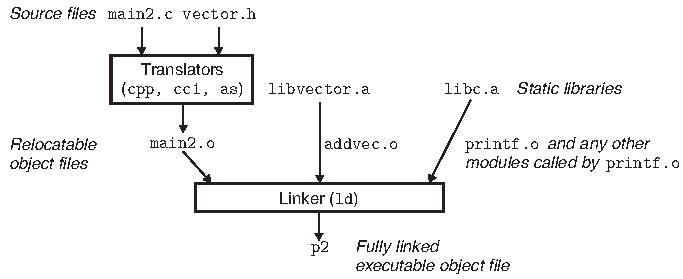
\includegraphics[width=\textwidth]{static-linking}
    } \mode<article>{
      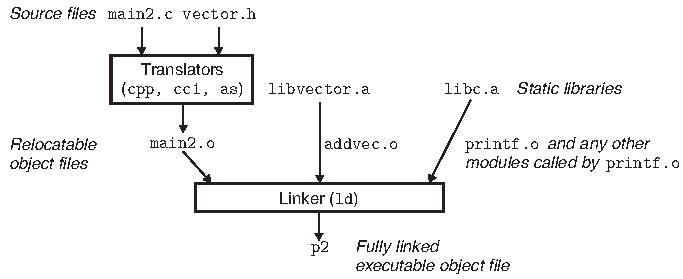
\includegraphics[width=.7\textwidth]{static-linking}
    }
  \end{center}
\end{frame}

% \begin{frame}{Dynamic Loading}
%   \begin{block}{Better memory utilization}
%     \begin{itemize}
%     \item Only the main program is loaded into memory and is executed
%     \item Routine is not loaded until it is called
%     \item Unused routine is never loaded
%     \item Useful when large amounts of code are needed to handle infrequently occurring
%       cases
%     \end{itemize}
%   \end{block}
%   \begin{center}
%     \mode<beamer>{
%       \includegraphics[width=.7\textwidth]{mm-dynamic}
%     } \mode<article>{
%       \includegraphics[width=.4\textwidth]{mm-dynamic}
%     }
%   \end{center}
% \end{frame}

\begin{frame}{Dynamic Linking}
  A \alert{dynamic linker} is actually a special loader that loads external shared
  libraries into a running process
  \begin{itemize}
    % \item Similar to dynamic loading
  \item Small piece of code, \texttt{stub}, used to locate the appropriate memory-resident
    library routine
  \item Only one copy in memory
  \item Don't have to re-link after a library update
  \end{itemize}
  \begin{center}
    \mode<beamer>{ \includegraphics[width=.8\textwidth]{mm-dynamic-linking} }
    \mode<article>{ \includegraphics[width=.4\textwidth]{mm-dynamic-linking} }
  \end{center}
\end{frame}

\begin{frame}{Dynamic Linking}
  \begin{center}
    \mode<beamer>{ 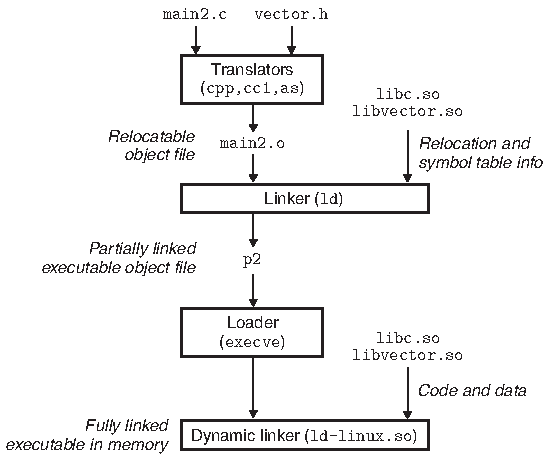
\includegraphics[width=.75\textwidth]{dynamic-linking2} }%
    \mode<article>{ 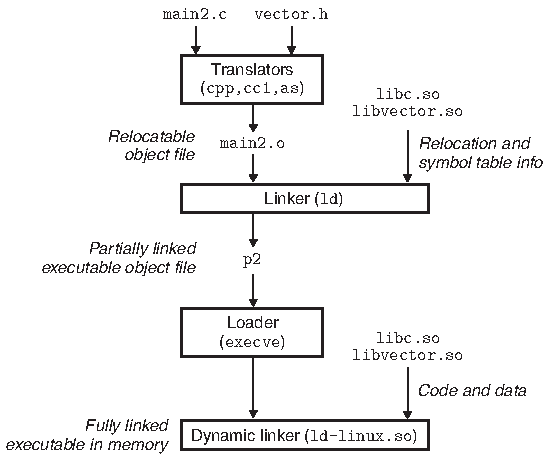
\includegraphics[width=.6\textwidth]{dynamic-linking2} }
  \end{center}
\end{frame}

\paragraph{More about dynamic linking}

Many operating system environments allow dynamic linking, that is the postponing of the
resolving of some undefined symbols until a program is run. That means that the executable
code still contains undefined symbols, plus a list of objects or libraries that will
provide definitions for these. Loading the program will load these objects/libraries as
well, and perform a final linking. Dynamic linking needs no linker\citetitle{wiki:linker}.

This approach offers two advantages:
\begin{itemize}
\item Often-used libraries (for example the standard system libraries) need to be stored
  in only one location, not duplicated in every single binary.
\item If an error in a library function is corrected by replacing the library, all
  programs using it dynamically will benefit from the correction after restarting
  them. Programs that included this function by static linking would have to be re-linked
  first.
\end{itemize}

There are also disadvantages:
\begin{itemize}
\item Known on the Windows platform as "DLL Hell", an incompatible updated DLL will break
  executables that depended on the behavior of the previous DLL.
\item A program, together with the libraries it uses, might be certified (e.g. as to
  correctness, documentation requirements, or performance) as a package, but not if
  components can be replaced. (This also argues against automatic OS updates in critical
  systems; in both cases, the OS and libraries form part of a qualified environment.)
\end{itemize}

% \subsubsection{Library Files}
% \label{sec:library-files}

\begin{frame}{Library Files}
  \begin{description}
  \item[Static libraries] \alert{\texttt{.a}} files. Very old ones, but still alive.
    \begin{itemize}
    \item[\$] \texttt{find /usr/lib -name "*.a"}
    \end{itemize}
  \item[Shared libraries] \alert{\texttt{.so}} files. The preferred ones.
    \begin{itemize}
    \item[\$] \texttt{find /usr/lib -name "*.so.*"}
    \end{itemize}
  \end{description}
  Examples:
  \begin{itemize}
  \item[\$] \texttt{gcc -o hello hello.c /usr/lib/libm.a}
  \item[\$] \texttt{gcc -o hello hello.c -lm}
  \end{itemize}
\end{frame}

\begin{frame}{Build A Static Library}{Source codes}
  \begin{minipage}[t]{.47\linewidth}
    \begin{block}{\texttt{main.c}}
      \begin{center}
        \mode<beamer>{ \includegraphics[width=\textwidth]{main-c} }%
        \mode<article>{\cfile{../src/mm/hello/static/main.c}}
      \end{center}
    \end{block}
    \begin{block}{\texttt{lib.h}}
      \mode<beamer>{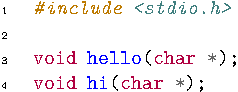
\includegraphics[width=.5\textwidth]{lib-h}}%
      \mode<article>{\cfile{../src/mm/hello/static/lib.h}}
    \end{block}
  \end{minipage}\qquad
  \begin{minipage}[t]{.43\linewidth}
    \begin{block}{\texttt{hello.c}}
      \begin{center}
        \mode<beamer>{ \includegraphics[width=\textwidth]{hello-c} }%
        \mode<article>{\cfile{../src/mm/hello/static/hello.c}}
      \end{center}
    \end{block}
    \begin{block}{\texttt{hi.c}}
      \begin{center}
        \mode<beamer>{ 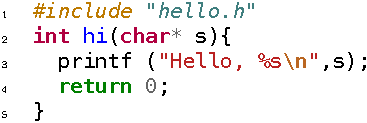
\includegraphics[width=\textwidth]{hi-c} }%
        \mode<article>{\cfile{../src/mm/hello/static/hi.c}}
      \end{center}
    \end{block}
  \end{minipage}
\end{frame}

\begin{frame}{Build A Static Library}{Step by step}
  \begin{enumerate}
  \item Get \alert{\texttt{hello.o}} and \alert{\texttt{hi.o}}
    \begin{itemize}
    \item[\$] \texttt{gcc -c hello.c hi.c}
    \end{itemize}
  \item Put \alert{\texttt{*.o}} into \alert{\texttt{libhi.a}}
    \begin{itemize}
    \item[\$] \texttt{ar crv libhi.a hello.o hi.o}
    \end{itemize}
  \item Use \alert{\texttt{libhi.a}}
    \begin{itemize}
    \item[\$] \texttt{gcc main.c libhi.a}
    \end{itemize}
  \end{enumerate}
\end{frame}

\begin{frame}{Build A Static Library}{Makefile}
  \begin{center}
    \mode<beamer>{ \includegraphics[width=.8\textwidth]{makefile-a} }%
    \mode<article>{\mkfile{../src/mm/hello/static/Makefile}}
  \end{center}
\end{frame}

\begin{frame}{Build A Shared Library}{Source codes}
  \begin{block}{\texttt{hello.c}}
    \begin{center}
      \mode<beamer>{ \includegraphics[width=.8\textwidth]{hello-c-so} }%
      \mode<article>{\cfile{../src/mm/hello/shared/hello.c}}
    \end{center}
  \end{block}
  \begin{minipage}{.35\linewidth}
    \begin{block}{\texttt{hello.h}}
      \mode<beamer>{ \includegraphics[width=\textwidth]{hello-h-so} }%
      \mode<article>{\cfile{../src/mm/hello/shared/hello.h}}
    \end{block}
  \end{minipage}\qquad
  \begin{minipage}{.36\linewidth}
    \begin{block}{\texttt{hi.c}}
      \mode<beamer>{ \includegraphics[width=\textwidth]{hi-c-so} }%
      \mode<article>{\cfile{../src/mm/hello/shared/hi.c}}
    \end{block}
  \end{minipage}
\end{frame}

\begin{frame}{Build A Shared Library}{Step by step}
  \begin{enumerate}
  \item Get \alert{\texttt{hi.o}}
    \begin{itemize}
    \item[\$] \texttt{gcc -fPIC -c hi.c}
    \end{itemize}
  \item Get \alert{\texttt{libhi.so}}
    \begin{itemize}
    \item[\$] \texttt{gcc -shared -o libhi.so hi.o}
    \end{itemize}
  \item Use \alert{\texttt{libhi.so}}
    \begin{itemize}
    \item[\$] \texttt{gcc -L. -Wl,-rpath=. hello.c -lhi}
    \end{itemize}
  \item Check it
    \begin{itemize}
    \item[\$] \texttt{ldd a.out}
    \end{itemize}
  \end{enumerate}
\end{frame}

\begin{frame}{Build A Shared Library}{Makefile}
  \begin{center}
    \mode<beamer>{ \includegraphics[width=\textwidth]{makefile-so} }%
    \mode<article>{\mkfile{../src/mm/hello/shared/Makefile}}
  \end{center}
\end{frame}

\begin{frame}{GNU C Library}
  \begin{minipage}{.55\linewidth}
    Linux API > POSIX API
    \ttfamily
    \begin{itemize}
    \item[\$] man 7 libc
    \item[\$] man 3 intro
    \item[\$] man gcc
    \item[\$] info gcc
    \item[\debian] sudo apt install gcc-doc
    \end{itemize}
  \end{minipage}
  \begin{minipage}{.4\linewidth}
    \begin{center}
      \mode<beamer>{ 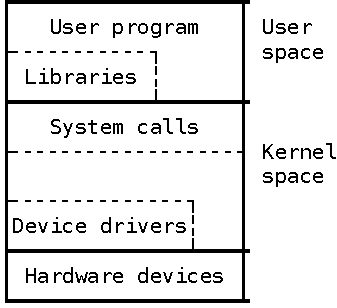
\includegraphics[width=\textwidth]{api} }%
      \mode<article>{ 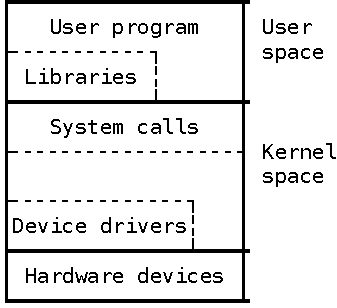
\includegraphics[width=.5\textwidth]{api} }
    \end{center}
  \end{minipage}
\end{frame}

\begin{frame}{Logical vs. Physical Address Space}
  \begin{itemize}
  \item Mapping logical address space to physical address space is central to MM
    \begin{description}
    \item[Logical address] generated by the CPU; also referred to as \alert{virtual
        address}
    \item[Physical address] address seen by the memory unit
    \end{description}
  \item In compile-time and load-time address binding schemes, LAS and PAS are identical
    in size
  \item In execution-time address binding scheme, they are differ.
  \end{itemize}
\end{frame}

\begin{frame}{Logical vs. Physical Address Space}%{Memory-Management Unit (MMU)}
  % \begin{itemize}
  % % \item Hardware device that maps virtual to physical address
  % % \item In MMU scheme, the value in the \textcolor{blue}{relocation (base) register
  % % } is added to every address generated by a user process at the time it is sent to
  % %   memory
  % \item The user program deals with logical addresses; it never sees the real physical
  %   addresses
  % \end{itemize}
  The user program
  \begin{itemize}
  \item deals with logical addresses
  \item never sees the real physical addresses
  \end{itemize}
  \begin{center}
    \mode<beamer>{ 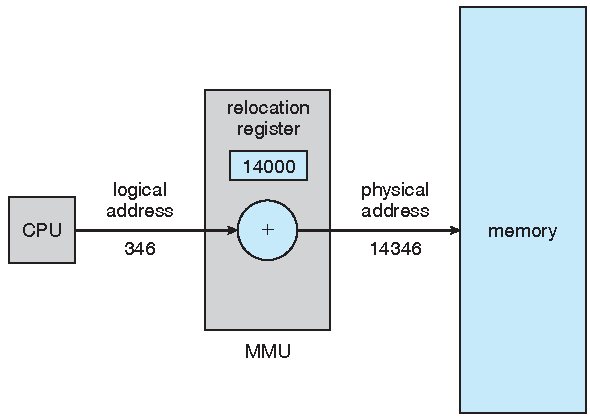
\includegraphics[width=.7\textwidth]{osc-8-10} }%
    \mode<article>{ 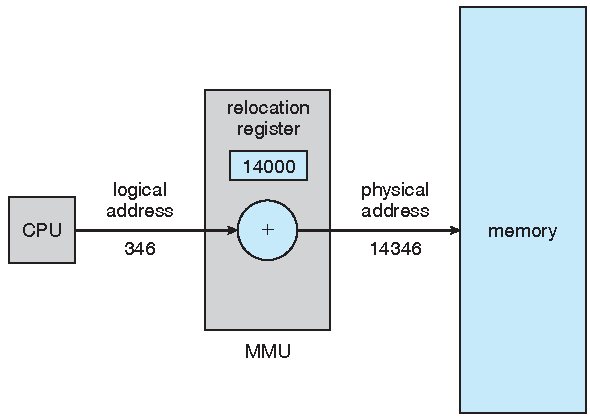
\includegraphics[width=.4\textwidth]{osc-8-10} }
  \end{center}
\end{frame}

\begin{frame}{MMU}{Memory Management Unit}
  \begin{center}
    \mode<beamer>{ 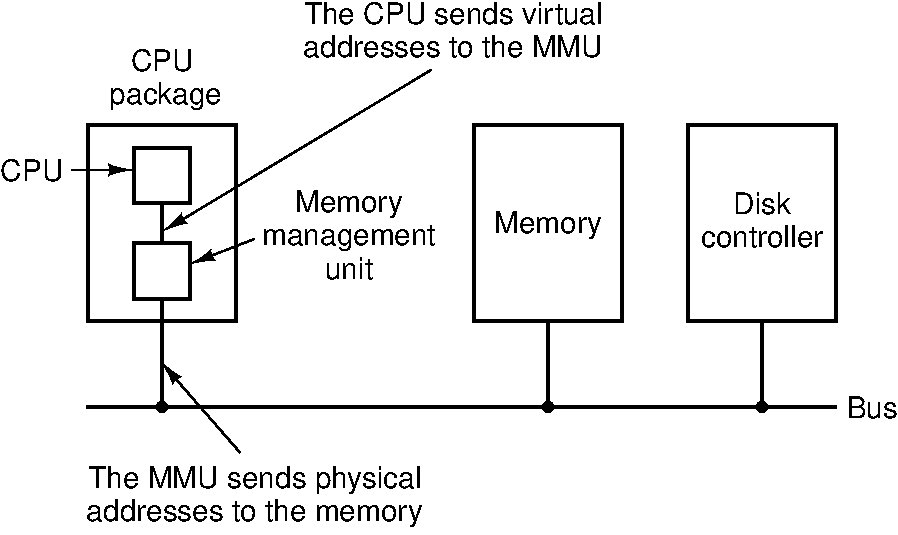
\includegraphics[width=\textwidth]{mos-figs-4-9} }%
    \mode<article>{ 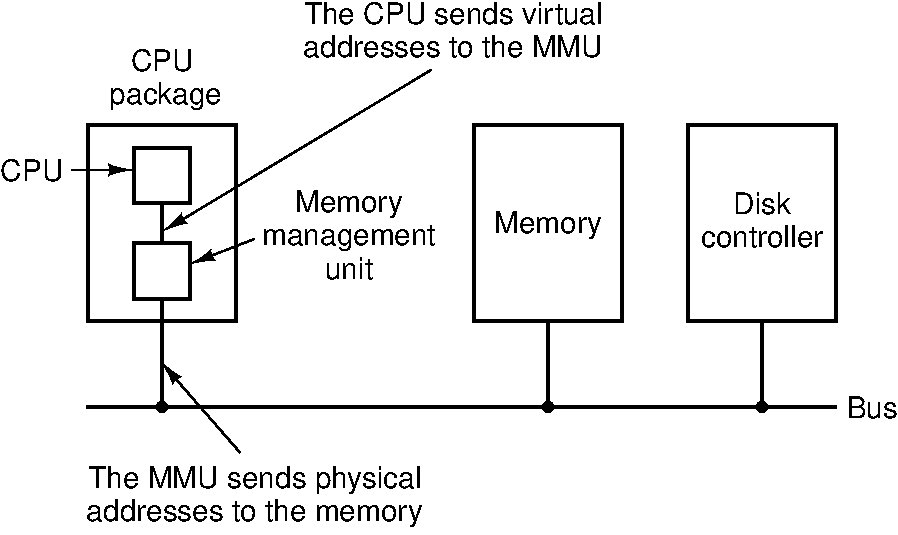
\includegraphics[width=.4\textwidth]{mos-figs-4-9} }
  \end{center}
\end{frame}

\begin{frame}{Memory Protection}
  \begin{center}
    \mode<beamer>{ 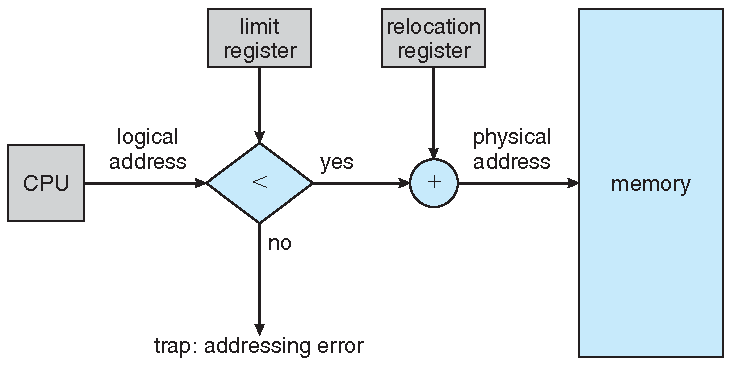
\includegraphics[width=\textwidth]{osc-8-16} }%
    \mode<article>{ 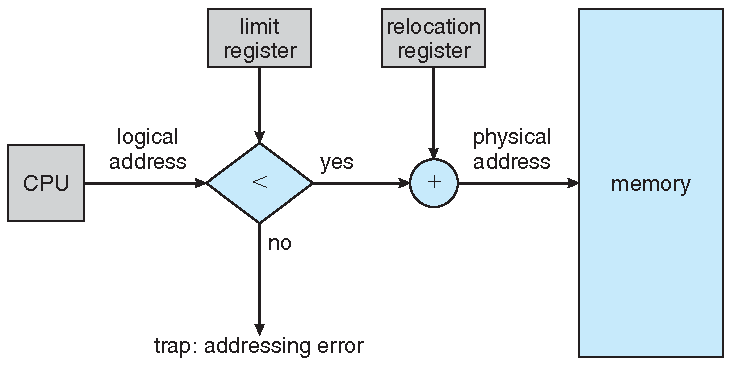
\includegraphics[width=.4\textwidth]{osc-8-16} }
  \end{center}
  % \begin{center}
  %   \hyperlink{reg}{Where are the \emph{base} and \emph{limit} registers from?}
  % \end{center}
\end{frame}

\begin{frame}{Swapping}
  \begin{center}
    \mode<beamer>{ 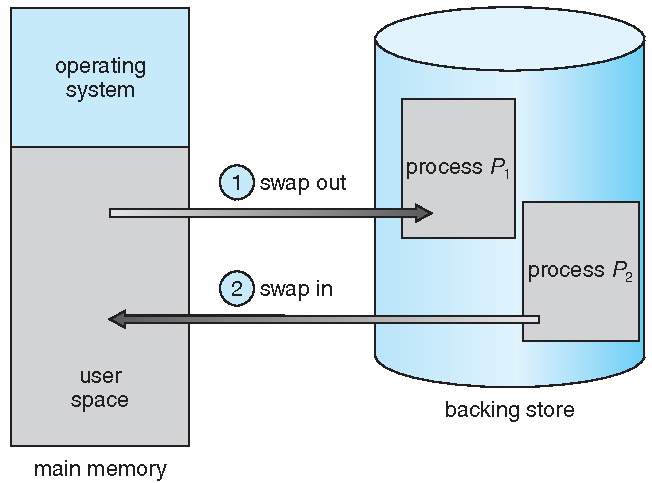
\includegraphics[width=.7\textwidth]{osc-8-14} }%
    \mode<article>{ 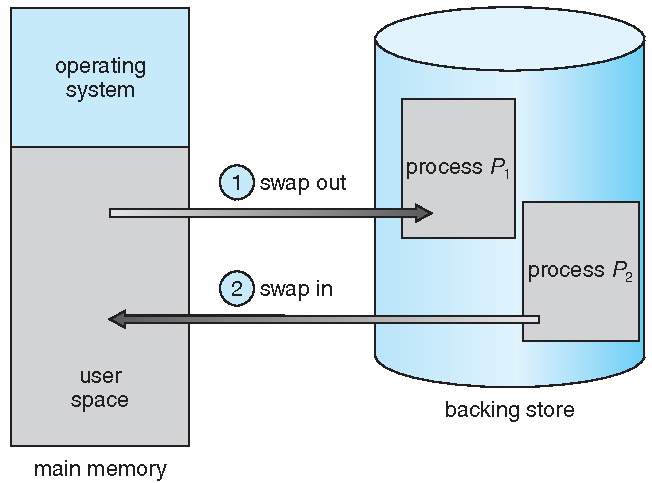
\includegraphics[width=.4\textwidth]{osc-8-14} }
  \end{center}
  \begin{block}{Major part of swap time is transfer time}
    \begin{itemize}
    \item[] Total transfer time is directly proportional to the amount of memory swapped
    \end{itemize}
  \end{block}
  % \item System maintains a ready queue of ready-to-run processes which have memory
  %   images on disk
\end{frame}

\section{Contiguous Memory Allocation}

\begin{frame}{Contiguous Memory Allocation}{Multiple-partition allocation}
  \begin{center}
    \mode<beamer>{ 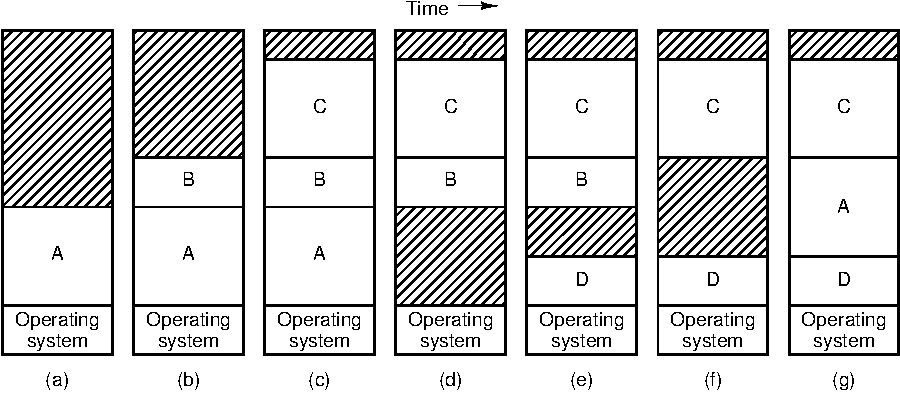
\includegraphics[width=\textwidth]{mos-figs-4-5} }%
    \mode<article>{ 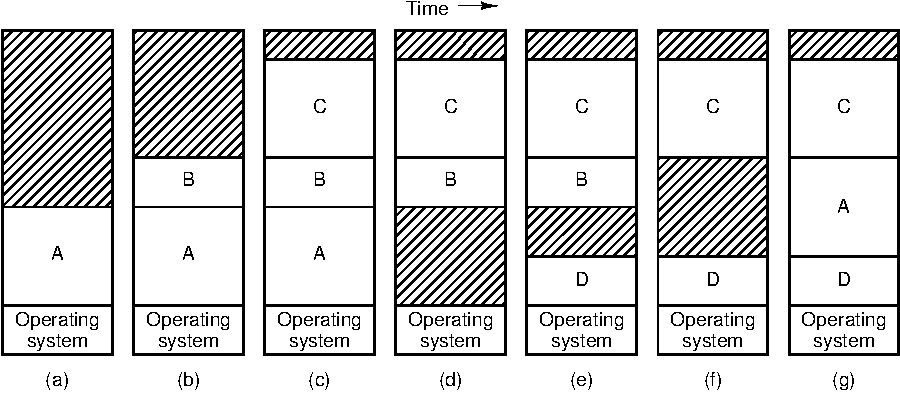
\includegraphics[width=.7\textwidth]{mos-figs-4-5} }
  \end{center}
  Operating system maintains information about:
  \begin{itemize}
  \item[a] allocated partitions
  \item[b] free partitions (hole)
  \end{itemize}
\end{frame}

\begin{frame}{Dynamic Storage-Allocation Problem}{First Fit, Best Fit, Worst Fit}
  \begin{center}
    \mode<beamer>{ \includegraphics[width=\textwidth]{mm-fit} }%
    \mode<article>{ \includegraphics[width=.4\textwidth]{mm-fit} }
  \end{center}
\end{frame}

\begin{frame}%{Dynamic Storage-Allocation Problem}
  \begin{description}
  \item[First-fit:] The first hole that is big enough
  \item[Best-fit:] The smallest hole that is big enough
    \begin{itemize}
    \item Must search entire list, unless ordered by size
    \item Produces the smallest leftover hole
    \end{itemize}
  \item[Worst-fit:] The largest hole
    \begin{itemize}
    \item Must also search entire list
    \item Produces the largest leftover hole
    \end{itemize}
  \end{description}
  \begin{itemize}
  \item First-fit and best-fit better than worst-fit in terms of speed and storage
    utilization
  \item First-fit is generally faster
  \end{itemize}
\end{frame}

\begin{frame}{Fragmentation}
  \begin{varwidth}{.3\textwidth}
    \includegraphics[width=\textwidth]{mm-frag}
  \end{varwidth}\hfill
  \begin{varwidth}{.66\textwidth}
    \begin{block}{Reduce external fragmentation by}
      \begin{itemize}
      \item \alert{Compaction} is possible only if relocation is dynamic,
        and is done at execution time
      \item \alert{Noncontiguous memory allocation}
        \begin{itemize}
        \item Paging
        \item Segmentation
        \end{itemize}
      \end{itemize}
    \end{block}
  \end{varwidth}
\end{frame}

\section{Virtual Memory}

\begin{frame}{Virtual Memory}{Logical memory can be much larger than physical memory}
  \begin{varwidth}{.48\textwidth}
    \begin{center}
      \mode<beamer>{ 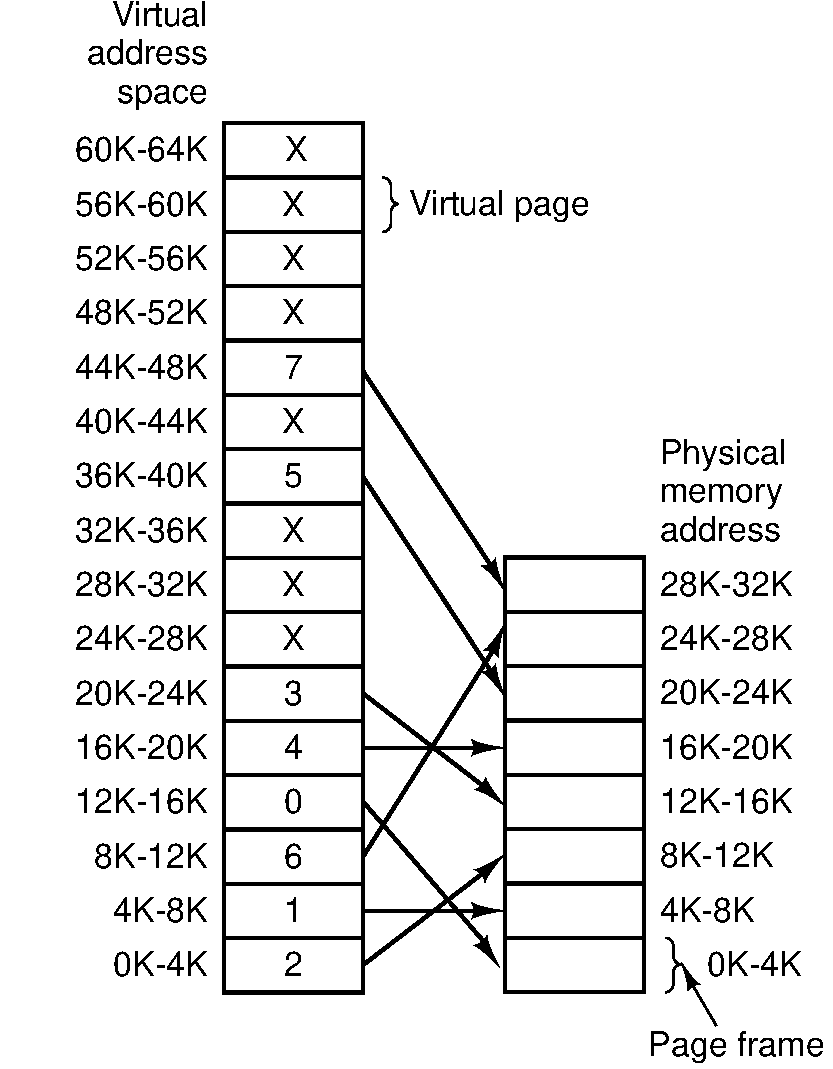
\includegraphics[width=\textwidth]{mos-figs-4-10} }%
      \mode<article>{ 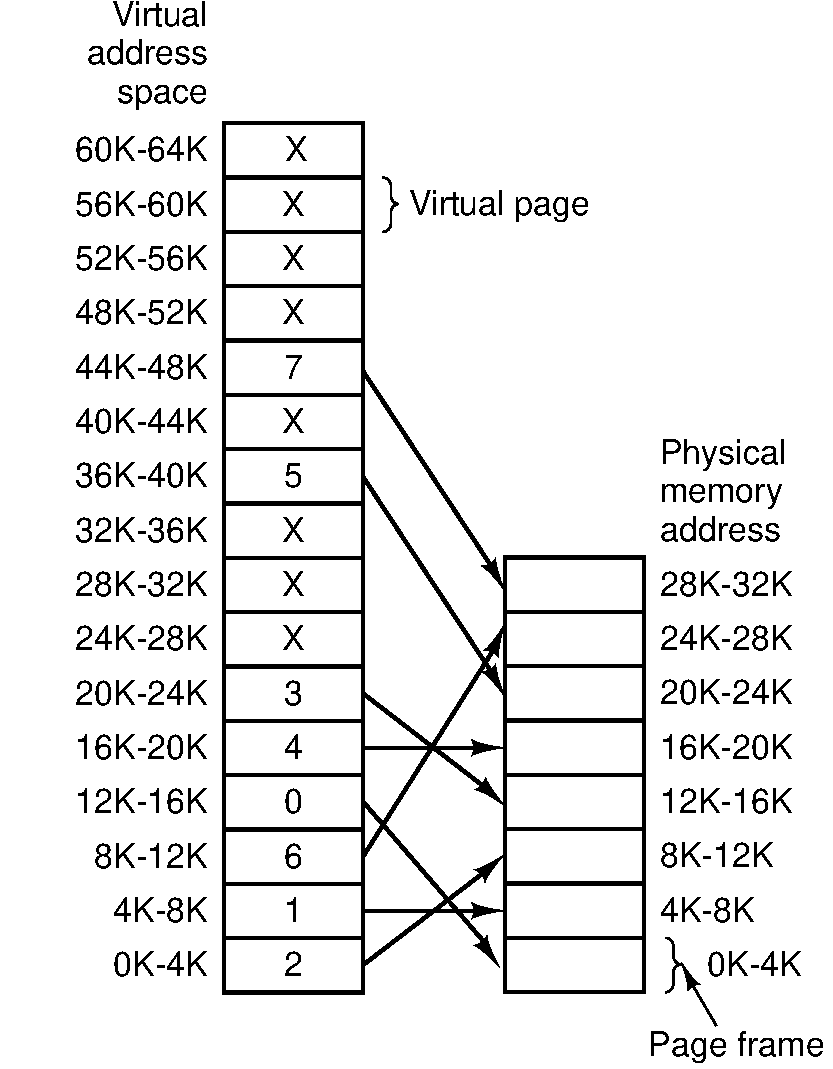
\includegraphics[width=.8\textwidth]{mos-figs-4-10} }
    \end{center}
  \end{varwidth}\hfill
  \begin{varwidth}{.48\textwidth}
    \begin{block}{Address translation}
      $$\genfrac{}{}{0pt}{}{virtual}{address}
      \xrightarrow{\alert{page\,table}}
      \genfrac{}{}{0pt}{}{physical}{address}$$
      
      $$Page\ 0\xrightarrow{map\,to}Frame\ 2$$
      
      $$0_{virtual}\xrightarrow{map\,to}8192_{physical}$$
      
      $$\genfrac{}{}{0pt}{}{20500_{vir}}{(20k+20)_{vir}}
      \xrightarrow{map\,to} \genfrac{}{}{0pt}{}{12308_{phy}}{(12k+20)_{phy}}$$
    \end{block}
  \end{varwidth}
\end{frame}

% \begin{frame}{Virtual Memory}{Memory Mapping}
%   \begin{center}
%     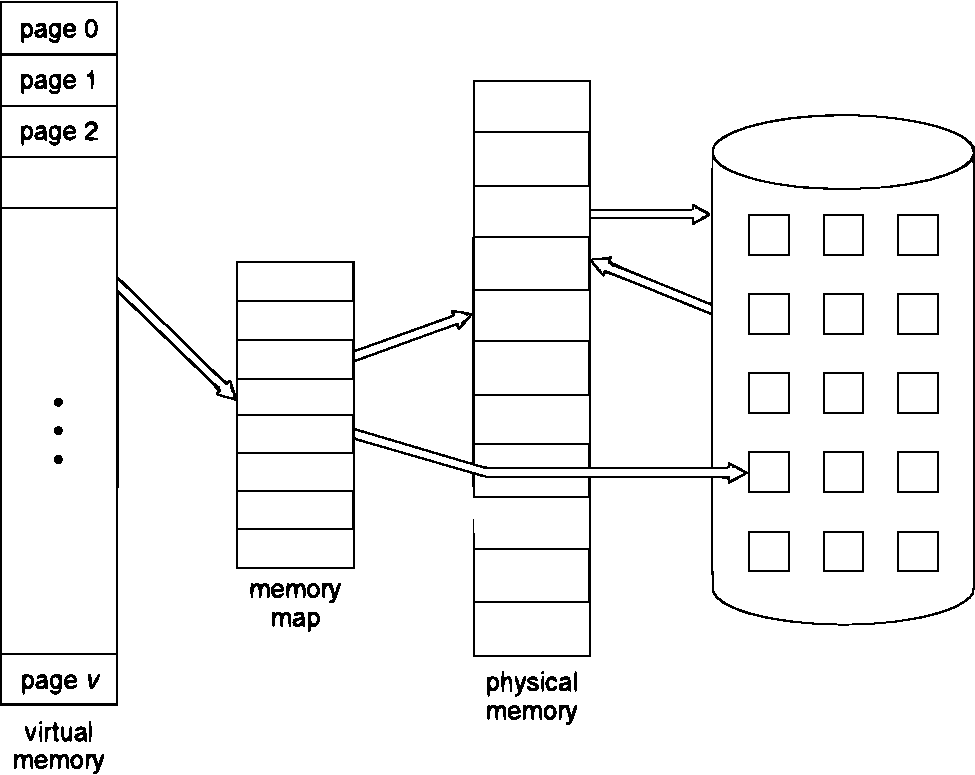
\includegraphics[width=.8\textwidth]{osc-9-5}
%   \end{center}
% \end{frame}

\subsection{Paging}

\begin{frame}{Paging}{Address Translation Scheme}
  \begin{block}{Address generated by CPU is divided into:}
    \begin{description}
    \item[Page number(p):] an index into a \emph{page table}
    \item[Page offset(d):] to be copied into memory
    \end{description}
  \end{block}
  Given \alert{logical address space} ($2^m$) and \alert{page size} ($2^n$),
  \begin{small}
    $$\text{number of pages}=\frac{2^m}{2^n}=2^{m-n}$$
  \end{small}
  \begin{block}{Example: addressing to $0010000000000100$}
    $$\underbrace{\overbrace{0\,0\,1\,0}^{m-n=4}\,\overbrace{0\,0\,0\,0\,0\,0\,0\,0\,0\,1\,0\,0}^{n=12}}_{m=16}$$
    \begin{small}
      $$\text{page number}=0010=2, \quad \text{page offset}=000000000100$$
    \end{small}
  \end{block}
\end{frame}

\begin{frame}
  \begin{varwidth}{.65\textwidth}
    \begin{center}
      \mode<beamer>{ 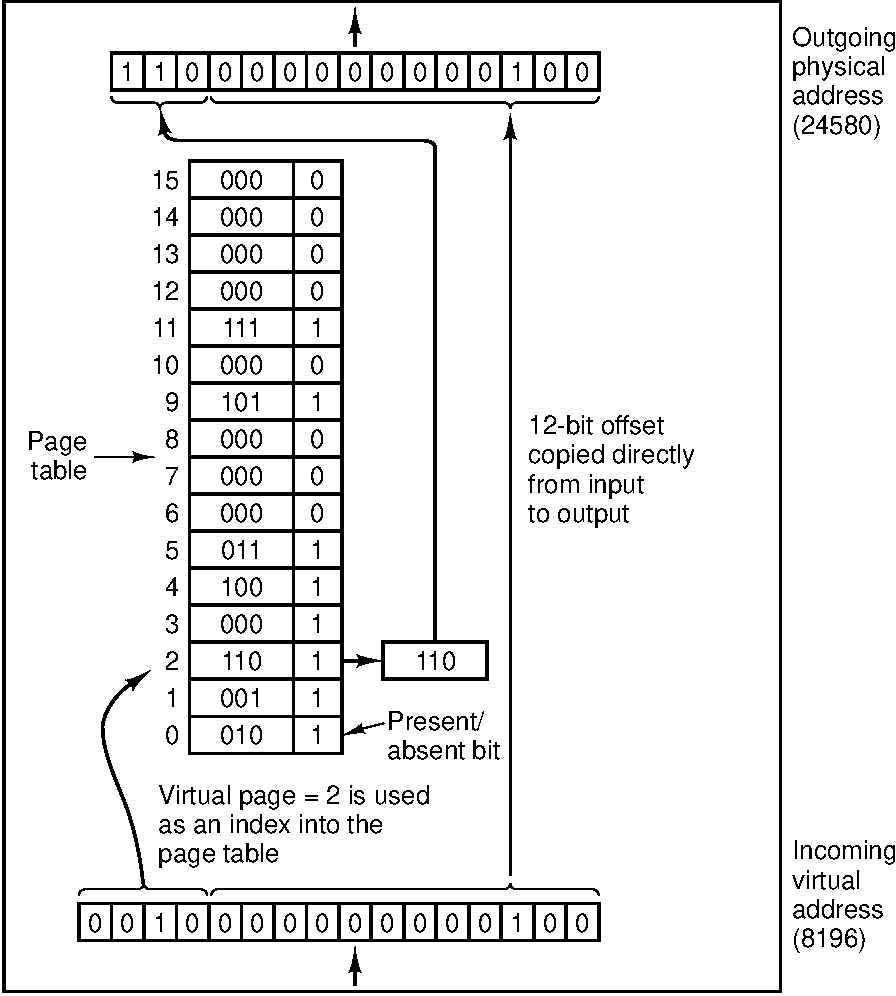
\includegraphics[width=\textwidth]{mos-figs-4-11} }%
      \mode<article>{ \includegraphics[width=.8\textwidth]{mos-figs-4-11} }
    \end{center}
    \label{fig:paging}
  \end{varwidth}\hfill
  \begin{varwidth}{.35\textwidth}
    \begin{small}
      \begin{tabular}{rl}
        Virtual pages:  &16\\
        Page size:      &4k\\
        Virtual memory:& 64K\\
        Physical frames:&8\\
        Physical memory:&32K
      \end{tabular}
    \end{small}
  \end{varwidth}
\end{frame}

% \begin{frame}{Valid-Invalid Bit}{When Some Pages Are Not In Memory}
%   \begin{center}
%     \mode<beamer>{ \includegraphics[width=.7\textwidth]{osc-9-11} }%
%     \mode<article>{ \includegraphics[width=.4\textwidth]{osc-9-11} }%
%   \end{center}
% \end{frame}

\begin{frame}[fragile]{Page Fault}
  \begin{varwidth}{.48\textwidth}
    \begin{center}
      \mode<beamer>{ \includegraphics[width=\textwidth]{mos-figs-4-10} }%
      \mode<article>{ \includegraphics[width=.8\textwidth]{mos-figs-4-10} }
    \end{center}
  \end{varwidth}\hfill
  \begin{varwidth}{.48\textwidth}
    \mintinline{nasm}|MOV REG, 32780|?
    \begin{itemize}
    \item[\Symbol{➠}] Page fault \& swapping
    \end{itemize}
  \end{varwidth}
\end{frame}

\begin{frame}{Page Fault Handling}
  \begin{center}
    \mode<beamer>{ \includegraphics[width=.8\textwidth]{osc-9-14} }%
    \mode<article>{ \includegraphics[width=.4\textwidth]{osc-9-14} }
  \end{center}
\end{frame}

% \begin{frame}{Free Frames}
%   \begin{center}
%     \includegraphics[width=.9\textwidth]{osc-8-25}\\
%     \begin{small}
%       before allocation \qquad\qquad\qquad\qquad after allocation
%     \end{small}
%   \end{center}
% \end{frame}

\begin{frame}{Shared Pages}
  \begin{center}
    \mode<beamer>{ \includegraphics[width=.7\textwidth]{osc-8-33} }%
    \mode<article>{ \includegraphics[width=.4\textwidth]{osc-8-33} }
  \end{center}
\end{frame}

\begin{frame}{Page Table Entry}{Intel i386 Page Table Entry}
  \begin{itemize}
  \item Commonly 4 bytes (32 bits) long
  \item Page size is usually 4k ($2^{12}$ bytes). OS dependent
    \begin{itemize}
    \item[\$] \texttt{getconf PAGESIZE}
    \end{itemize}
  \item Could have $2^{32-12}=2^{20}=1M$ pages
    \begin{itemize}
    \item[] Could address $1M\times{}4KB=4GB$ memory
    \end{itemize}
  \end{itemize}
  \begin{center}
    \mode<beamer>{ \includegraphics[width=\textwidth]{i386pte} }%
    \mode<article>{ \includegraphics[width=.5\textwidth]{i386pte} }
  \end{center}
\end{frame}

\begin{frame}{Page Table}
  \begin{itemize}
  \item Page table is kept in main memory
  \item Usually one page table for each process
  \item \alert{Page-table base register (PTBR):} A pointer to the page table is stored in
    PCB
  \item \alert{Page-table length register (PRLR):} indicates size of the page table
  \item Slow
    \begin{itemize}
    \item Requires two memory accesses. One for the page table and one for the
      data/instruction.
    \end{itemize}
  \item TLB
  \end{itemize}
\end{frame}

\begin{frame}{Translation Lookaside Buffer (TLB)}
  \begin{description}
  \item[80-20 rule] Only a small fraction of the PTEs are heavily read; the rest are
    barely used at all
  \end{description}
  \begin{center}
    \mode<beamer>{ \includegraphics[width=.7\textwidth]{osc-8-28} }%
    \mode<article>{ \includegraphics[width=.5\textwidth]{osc-8-28} }
  \end{center}
\end{frame}

\begin{frame}{Multilevel Page Tables}
%  \begin{minipage}{.54\textwidth}
    \begin{itemize}
    \item a $1M$-entry page table eats $4M$ memory
    \item while 100 processes running, $400M$ memory is gone for page tables
    \item avoid keeping all the page tables in memory all the time
    \end{itemize}
    \begin{block}{A two-level scheme}
      \begin{center}
        \mode<beamer>{ \includegraphics[width=.6\textwidth]{2-level-paging} }%
        \mode<article>{ \includegraphics[width=.3\textwidth]{2-level-paging} }
      \end{center}
    \end{block}    
    %  \end{minipage}\hfill
  % \begin{minipage}{.46\textwidth}
  %   \begin{center}
  %     \mode<beamer>{ \includegraphics[width=\textwidth]{osc-8-36} }%
  %     \mode<article>{ \includegraphics[width=.8\textwidth]{osc-8-36} }
  %   \end{center}
  %   \label{fig:2levelpaging}
  % \end{minipage}
\end{frame}

\begin{description}
\item[p1:] is an index into the outer page table
\item[p2:] is the displacement within the page of the outer page table
\end{description}

\begin{itemize}
\item Split one huge page table into 1k small page tables
  \begin{itemize}
  \item i.e. the huge page table has 1k entries.
  \item Each entry keeps a page frame number of a small page table.
  \end{itemize}
\item Each small page table has 1k entries
  \begin{itemize}
  \item Each entry keeps a page frame number of a physical frame.
  \end{itemize}
\end{itemize}

% \begin{frame}{Two-level Page-Table Scheme}
%   \begin{center}
%     %     \includegraphics[width=\textwidth]{osc-8-38}
%     \begin{center}
%       \includegraphics[width=\textwidth]{two-level-paging}
%     \end{center}

%   \end{center}
%   %   \begin{small}
%   %   \begin{itemize}
%   %   \item[$P_1$] is an index into the outer page table
%   %   \item[$P_2$] is the displacement within the page of the outer page table
%   %   \end{itemize}
%   % \end{small}
% \end{frame}

% \begin{frame}{Memory protection}
%   \begin{itemize}
%   \item Protection bit --- R/W
%   \item \textcolor{blue}{Valid-invalid} bit
%     \begin{itemize}
%     \item Many processes use only a small fraction of the address space available to
%       them
%     \item "valid" indicates that the associated page is in the process' logical address
%       space, and is thus a legal page
%     \item "invalid" indicates that the page is not in the process' logical address space
%     \end{itemize}
%   \end{itemize}
% \end{frame}

% \begin{frame}{Valid (v) or Invalid (i) Bit}
%   \begin{center}
%     \includegraphics[width=.9\textwidth]{osc-8-31}
%   \end{center}
% \end{frame}

\begin{frame}{Two-Level Page Tables}{Example}
  \begin{center}
    \mode<beamer>{ \includegraphics[width=.8\textwidth]{2-level-paging-2} }%
    \mode<article>{ \includegraphics[width=.6\textwidth]{2-level-paging-2} }
  \end{center}
  % \begin{minipage}{.3\linewidth}
  %   \mbox{Don't have to keep all the $1K$ page tables} \mbox{($1M$ pages) in memory. In
  %     this example} \mbox{only 4 page tables are actually} \mbox{mapped into memory}\\[1ex]
  %   \begin{center}
  %     \includegraphics[width=.7\textwidth]{process}
  %   \end{center}
  % \end{minipage}\hfill
  % \begin{minipage}{.68\linewidth}
  %   \includegraphics[width=\textwidth]{2-level-paging-2}%{mos-figs-4-12}
  % \end{minipage}
\end{frame}

\begin{frame}{Problem With 64-bit Systems}
  \begin{description}
  \item[Given:]\hfill\\[-2ex]
    \begin{itemize}
    \item $\text{virtual address space} = 64\,bits$
    \item $\text{page size}=4\,KB=2^{12}\,B$
    \end{itemize}
  \item[?] How much space would a simple single-level page table take?
    \begin{itemize}
    \item[if] Each page table entry takes $4\,Bytes$
    \item[then] The whole page table ($2^{64-12}$ entries) will take
      \[2^{64-12}\times{}4\,B=2^{54}\,B=16\,PB \quad {\scriptstyle(peta \Rightarrow tera \Rightarrow giga)!}\]
    \end{itemize}
    And this is for ONE process!
  \item[Multi-level?]\hfill
    \begin{itemize}
    \item[if] $10\,bits$ for each level
    \item[then] $\frac{64-12}{10}=5$ levels are required
    \end{itemize}
    5 memory accress for each address translation!
  \end{description}
\end{frame}

\begin{frame}{Inverted Page Tables}{Index with frame number}
  \begin{block}{Inverted Page Table:}
    \begin{itemize}
    \item One entry for each \emph{physical} frame
      \begin{itemize}
      \item The physical frame number is the table index
      \end{itemize}
    \item A single global page table for all processes
      \begin{itemize}
      \item The table is shared --- PID is required
      \end{itemize}
    \end{itemize}
  \end{block}
  \begin{itemize}
  \item Physical pages are now mapped to virtual --- each entry contains a virtual page
    number instead of a physical one
  \item Information bits, e.g. protection bit, are as usual
  \end{itemize}
\end{frame}

\begin{frame}
  \begin{block}{Find index according to entry contents}
    $(pid,\,p)\Rightarrow{}i$
    \begin{center}
      \mode<beamer>{ \includegraphics[width=.8\textwidth]{osc-8-43} }%
      \mode<article>{ \includegraphics[width=.5\textwidth]{osc-8-43} }
    \end{center}
  \end{block}
\end{frame}

\begin{frame}%{Linear Inverted Page Tables}
  \begin{minipage}[t]{.39\linewidth}
    Std. PTE (32-bit sys.):
    \begin{center}
      \mode<beamer>{ \includegraphics[width=\textwidth]{pte1} }%
      \mode<article>{ \includegraphics[width=.7\textwidth]{pte1} }

      \scriptsize{indexed by page number}
    \end{center}
    \begin{itemize}
    \item[if] $2^{20}\,entries, 4\,B\text{ each}$
    \item[then] $SIZE_{page\,table}=2^{20}\times{}4 = 4\,MB$ \\(for \emph{each} process)
    \end{itemize}
  \end{minipage}
  \hfill
  \begin{minipage}[t]{.58\linewidth}
    Inverted PTE (64-bit sys.):
    \begin{center}
      \mode<beamer>{ \includegraphics[width=.88\textwidth]{pte2} }%
      \mode<article>{ \includegraphics[width=.6\textwidth]{pte2} }

      \scriptsize{indexed by frame number}
    \end{center}
    \begin{itemize}
    \item[if] assuming
      \begin{itemize}
      \item 16 bits for PID
      \item 52 bits for virtual page number
      \item 12 bits of information
      \end{itemize}
    \item[then] each entry takes $16 + 52 + 12 = 80\,bits = 10\,bytes$
    \item[if] $\text{physical mem}=1G\,(2^{30}\,B)$, and $\text{page
        size}=4K\,(2^{12}\,B)$, we'll have $2^{30-12} = 2^{18}\,pages$
    \item[then] $SIZE_{page\,table}=2^{18}\times{}10\,B=2.5\,MB$ \\(for \emph{all}
      processes)
    \end{itemize}
  \end{minipage}
\end{frame}

\begin{frame}
  \begin{description}
  \item[Inefficient:] Require searching the entire table 
  \end{description}
  \begin{center}
    \mode<beamer>{ \includegraphics[width=.9\textwidth]{ipt} }%
    \mode<article>{ \includegraphics[width=.4\textwidth]{ipt} }
  \end{center}
\end{frame}

\begin{frame}{Hashed Inverted Page Tables}
  \begin{description}
  \item[A hash anchor table] --- an extra level before the actual page table 
  \end{description}
  \begin{itemize}
    % \item at least as large as the page table
  \item maps
    \begin{scriptsize}
      \begin{tabular}{r}
        process IDs\\
        virtual page numbers
      \end{tabular}
    \end{scriptsize}
    $\Rightarrow{}$page table entries
  \item Since collisions may occur, the page table must do chaining
  \end{itemize}
  \begin{center}
    \mode<beamer>{ \includegraphics[width=.9\textwidth]{osc-8-41} }%
    \mode<article>{ \includegraphics[width=.4\textwidth]{osc-8-41} }
  \end{center}
\end{frame}

\begin{frame}{Hashed Inverted Page Table}
  \begin{center}
    \mode<beamer>{ \includegraphics[width=\textwidth]{ipt-hash} }%
    \mode<article>{ \includegraphics[width=.4\textwidth]{ipt-hash} }
  \end{center}
  % \includegraphics[width=\textwidth]{hash-table}
\end{frame}

\subsection{Demand Paging}

\begin{frame}{Demand Paging}
  \begin{block}{With demand paging, the size of the LAS is no longer constrained by
      physical memory}
    \begin{itemize}
    \item Bring a page into memory only when it is needed
      \begin{itemize}
      \item Less I/O needed
      \item Less memory needed
      \item Faster response
      \item More users
      \end{itemize}
    \item Page is needed $\Rightarrow$ reference to it
      \begin{itemize}
      \item invalid reference $\Rightarrow$ abort
      \item not-in-memory $\Rightarrow$ bring to memory
      \end{itemize}
    \item \alert{Lazy swapper} - never swaps a page into memory unless page will
      be needed
      \begin{itemize}
      \item \alert{Swapper} deals with entire processes
      \item \alert{Pager (Lazy swapper)} deals with pages
      \end{itemize}
    \end{itemize}
  \end{block}
\end{frame}

\paragraph{More about demand paging}

In the purest form of paging, processes are started up with none of their pages in
memory. As soon as the CPU tries to fetch the first instruction, it gets a page fault,
causing the operating system to bring in the page containing the first instruction. Other
page faults for global variables and the stack usually follow quickly. After a while, the
process has most of the pages it needs and settles down to run with relatively few page
faults. This strategy is called \emph{demand paging} because pages are loaded only on
demand, not in advance\citetitle[Sec.~3.4.8, P.~207]{tanenbaum2008modern}.

\subsection{Copy-on-Write}

\begin{frame}{Copy-on-Write}{More efficient process creation}
  \begin{varwidth}{.49\textwidth}
    \begin{itemize}
    \item Parent and child processes initially share the same pages in memory
    \item Only the modified page is copied upon modification occurs
    \item Free pages are allocated from a \emph{pool} of zeroed-out pages
    \end{itemize}
  \end{varwidth}\hfill
  \begin{varwidth}{.49\textwidth}
    \begin{center}
      \includegraphics[width=\textwidth]{osc-9-19}
    \end{center}
    \begin{center}
      \includegraphics[width=\textwidth]{osc-9-20}
    \end{center}
  \end{varwidth}
\end{frame}

\subsection{Memory mapped files}

\begin{frame}{Memory Mapped Files}
  \begin{center}
    Mapping a file (disk block) to one or more memory pages
  \end{center}
  \begin{minipage}{.49\textwidth}
    \begin{itemize}
    \item \alert{Improved I/O performance} --- much faster than \emph{read()}
      and \emph{write()} system calls
    \item \alert{Lazy loading (demand paging)} --- only a small portion of file
      is loaded initially
    \item A mapped file can be shared, like \emph{shared library}
    \end{itemize}
  \end{minipage}\quad
  \begin{minipage}{.45\textwidth}
    \includegraphics[width=1.15\textwidth]{osc-9-54}
  \end{minipage}
\end{frame}

\subsection{Page Replacement Algorithms}

\begin{frame}{Need For Page Replacement}
  \begin{description}
  \item[Page replacement:] find some page in memory, but not really in use, swap it out
  \end{description}
  \begin{center}
    \mode<beamer>{ \includegraphics[width=.8\textwidth]{osc-9-23} }%
    \mode<article>{ \includegraphics[width=.4\textwidth]{osc-9-23} }
  \end{center}
\end{frame}

Linux calls it the \emph{Page Frame Reclaiming
  Algorithm}\footnote{\url{http://stackoverflow.com/questions/5889825/page-replacement-algorithm}},
it's basically LRU with a bias towards non-dirty pages.

See also:
\begin{itemize}
\item \citetitle[\emph{Wikipedia: Page replacement algorithm}]{wiki:page-replace}.
\item \citetitle[Chap.~17, \emph{Page Frame Reclaiming}]{bovet2005understanding}.
\item PageReplacementDesign\footnote{\url{http://linux-mm.org/PageReplacementDesign}}.
\end{itemize}

\begin{frame}{Performance Concern}
  Because disk I/O is so expensive, we must solve two major problems to implement demand
  paging.
  \begin{description}
  \item[Frame-allocation algorithm] If we have multiple processes in memory, we must
    decide how many frames to allocate to each process.
  \item[Page-replacement algorithm] When page replacement is required, we must select the
    frames that are to be replaced.
  \end{description}
  \begin{block}{Performance}
    We want an algorithm resulting in lowest page-fault rate
    \begin{itemize}
    \item Is the victim page modified?
    \item Pick a random page to swap out?
    \item Pick a page from the faulting process' own pages? Or from others?
    \end{itemize}
  \end{block}
\end{frame}

\begin{frame}{Page-Fault Frequency Scheme}
  Establish "acceptable" page-fault rate
  \begin{center}
    \mode<beamer>{ \includegraphics[width=\textwidth]{osc-9-51} }
    \mode<article>{ \includegraphics[width=.4\textwidth]{osc-9-51} }
  \end{center}
\end{frame}

\begin{frame}{FIFO Page Replacement Algorithm}
  \begin{center}
    \mode<beamer>{ \includegraphics[width=\textwidth]{osc-9-29} }
    \mode<article>{ \includegraphics[width=.6\textwidth]{osc-9-29} }
  \end{center}
  \begin{itemize}
  \item Maintain a linked list (FIFO queue) of all pages
    \begin{itemize}
    \item in order they came into memory
    \end{itemize}
  \item Page at beginning of list replaced
  \item Disadvantage
    \begin{itemize}
    \item The oldest page may be often used
    \item Belady's anomaly
    \end{itemize}
  \end{itemize}
\end{frame}

\begin{frame}{FIFO Page Replacement Algorithm}{Belady's Anomaly}
  \begin{itemize}
  \item Reference string: 1, 2, 3, 4, 1, 2, 5, 1, 2, 3, 4, 5
  \item 3 frames (3 pages can be in memory at a time per process)
    \begin{center}
      \begin{tabular}{cccc}
        \fbox{1}&4&5&3\\
        \fbox{2}&1&\sout{1}&4\\
        \fbox{3}&2&\sout{2}&\sout{5}
      \end{tabular}\qquad
      9 page faults
    \end{center}
  \item 4 frames
    \begin{center}
      \begin{tabular}{ccc}
        \fbox{1}&\sout{1}&2\\
        \fbox{2}&\sout{2}&3\\
        \fbox{3}&5&4\\
        \fbox{4}&1&5
      \end{tabular}\qquad\quad
      10 page faults
    \end{center}
  \item Belady's Anomaly: \alert{more frames $\Rightarrow$ more page faults}
  \end{itemize}
\end{frame}

\begin{frame}{Optimal Page Replacement Algorithm (OPT)}
  \begin{center}
    \mode<beamer>{ \includegraphics[width=\textwidth]{osc-9-32} }
    \mode<article>{ \includegraphics[width=.6\textwidth]{osc-9-32} }
  \end{center}
  \begin{itemize}
  \item Replace page needed at the farthest point in future
    \begin{itemize}
    \item Optimal but not feasible
    \end{itemize}
  \item Estimate by ...
    \begin{itemize}
    \item logging page use on previous runs of process
    \item although this is impractical, similar to SJF CPU-scheduling, it can be used for
      comparison studies
    \end{itemize}
  \end{itemize}
\end{frame}

\begin{frame}{Least Recently Used (LRU) Algorithm}
  \begin{itemize}
  \item[FIFO] uses the time when a page was brought into memory
  \item[OPT] uses the time when a page is to be used
  \item[LRU] uses the recent past as an approximation of the near future
  \end{itemize}
  Replace the page that \emph{has not been used} for the longest period of time
  \begin{block}{Assume recently-used-pages will used again soon}
    \begin{center}
      \mode<beamer>{ \includegraphics[width=\textwidth]{osc-9-34} }%
      \mode<article>{ \includegraphics[width=.6\textwidth]{osc-9-34} }
    \end{center}
  \end{block}
\end{frame}

\begin{frame}{LRU Implementations}
  \begin{block}{\alert{Counters}: record the time of the last reference
      to each page}
    \begin{itemize}
    \item choose page with lowest value counter
    \item Keep counter in each page table entry
    \item counter overflow --- periodically zero the counter
    \item require a \alert{search} of the page table to find the LRU page
    \item update time-of-use field in the page table \alert{every memory reference!}
    \end{itemize}
  \end{block}
  \begin{block}{\alert{Stack}: keep a linked list (stack) of pages}
    \begin{itemize}
    \item most recently used at top, least (LRU) at bottom
      \begin{itemize}
      \item no search for replacement
      \end{itemize}
    \item whenever a page is referenced, it's removed from the stack and put on the top
      \begin{itemize}
      \item update this list \alert{every memory reference!}
      \end{itemize}
    \end{itemize}
  \end{block}
\end{frame}

\begin{frame}{Second Chance Page Replacement Algorithm}
  \begin{center}
    \mode<beamer>{
      \includegraphics[width=\textwidth]{mos-figs-4-17}
    }
    \mode<article>{
      \includegraphics[width=.6\textwidth]{mos-figs-4-17}
    }
  \end{center}
  % \begin{center}
  %   \includegraphics[width=.9\textwidth]{osc-9-38}
  % \end{center}
\end{frame}

\subsection{Allocation of Frames}

\begin{frame}{Allocation of Frames}
  \begin{itemize}
  \item Each process needs minimum number of pages
  \item Fixed Allocation
    \begin{itemize}
    \item Equal allocation --- e.g., 100 frames and 5 processes, give
      each process 20 frames.
    \item Proportional allocation --- Allocate according to the size of process
      $$a_i=\frac{s_i}{\sum{}s_i}\times{}m$$
      \begin{description}
      \item[$S_i$:] size of process $p_i$
      \item[$m$:] total number of frames
      \item[$a_i$:] frames allocated to $p_i$
      \end{description}
    \end{itemize}
  \item Priority Allocation --- Use a proportional allocation scheme
    using priorities rather than size
    $$\frac{priority_i}{\sum{}priority_i}\quad or\quad (\frac{s_i}{\sum{}s_i},\,\frac{priority_i}{\sum{}priority_i})$$
  \end{itemize}
\end{frame}

\begin{frame}{Global vs. Local Allocation}
  If process $P_i$ generates a page fault, it can select a replacement frame
  \begin{itemize}
  \item from its own frames --- \alert{Local replacement}
  \item from the set of all frames; one process can take a frame from another ---
    \alert{Global replacement}
    \begin{itemize}
    \item from a process with lower priority number
    \end{itemize}
  \end{itemize}
  \alert{Global replacement generally results in greater system throughput.}
\end{frame}

\subsection{Thrashing And Working Set Model}

\begin{frame}{Thrashing}
  \begin{center}
    \mode<beamer>{
      \includegraphics[width=\textwidth]{thrashing}
    }
    \mode<article>{
      \includegraphics[width=.4\textwidth]{thrashing}
    }
  \end{center}
\end{frame}

\begin{frame}{Thrashing}
  \begin{enumerate}
  \item CPU not busy $\Rightarrow$ add more processes
  \item a process needs more frames $\Rightarrow$ faulting, and taking frames away from
    others
  \item these processes also need these pages $\Rightarrow$ also faulting, and taking
    frames away from others $\Rightarrow$ chain reaction
  \item more and more processes queueing for the paging device $\Rightarrow$ ready queue
    is empty $\Rightarrow$ CPU has nothing to do $\Rightarrow$ add more processes
    $\Rightarrow$ more page faults
  \item MMU is busy, but no work is getting done, because processes are busy paging ---
    \alert{thrashing}
  \end{enumerate}
\end{frame}

\begin{frame}{Demand Paging and Thrashing}{Locality Model}
  \begin{minipage}{.5\textwidth}
    \begin{itemize}
    \item A \alert{locality} is a set of pages that are actively used together
    \item Process migrates from one locality to another
      % \item Localities may overlap
    \end{itemize}
  \end{minipage}\hfill
  \begin{minipage}{.4\textwidth}
    \begin{center}
      \mode<beamer>{
        \includegraphics[width=\textwidth]{osc-9-47}
      } \mode<article>{
        \includegraphics[width=.7\textwidth]{osc-9-47}
      }
      {\tiny locality in a memory reference pattern}
    \end{center}
  \end{minipage}
  
  \begin{description}
  \item[Why does thrashing occur?]
    \begin{small}
      $$\sum_{i=(0,n)}Locality_i > \textit{total memory size}$$
    \end{small}
  \end{description}
\end{frame}

\begin{frame}{Working-Set Model}
  \begin{description}
  \item[Working Set (WS)] The set of pages that a process is currently($\Delta$)
    using. ($\approx{}$locality)
  \end{description}
  \begin{center}
    \mode<beamer>{
      \includegraphics[width=.9\textwidth]{osc-9-49}
    } \mode<article>{
      \includegraphics[width=.6\textwidth]{osc-9-49}
    }
  \end{center}
  \begin{block}{}
    \begin{description}
    \item[$\Delta$:] Working-set window. In this example,
      \begin{itemize}
      \item[] $\Delta=10\ \texttt{memory access}$
      \end{itemize}
    \item[WSS:] Working-set size.  $WS(t_1)=\{\overbrace{1,\,2,\,5,\,6,\,7}^{WSS=5}\}$
    \end{description}
  \end{block}
  \begin{itemize}
  \item The accuracy of the working set depends on the selection of $\Delta$
  \item Thrashing, if $\sum{}WSS_i > SIZE_{total\,memory}$
  \end{itemize}
\end{frame}

\begin{frame}{The Working-Set Page Replacement Algorithm}
  \begin{block}{To evict a page that is not in the working set}
    \begin{center}
      \mode<beamer>{ \includegraphics[width=.9\textwidth]{mos-figs-4-21} }
      \mode<article>{ \includegraphics[width=.6\textwidth]{mos-figs-4-21} }
    \end{center}
    $$age = \textit{Current virtual time} - \textit{Time of last use}$$
  \end{block}
\end{frame}

\begin{description}
\item[Current virtual time] The amount of CPU time a process has actually used since it
  started is often called its \emph{current virtual time}\citetitle[sec~3.4.8,
  p~209]{tanenbaum2008modern}.
\end{description}

The algorithm works as follows. The hardware is assumed to set the \texttt{R} and
\texttt{M} bits, as discussed earlier. Similarly, a periodic clock interrupt is assumed to
cause software to run that clears the \texttt{Referenced} bit on every clock tick. On
every page fault, the page table is scanned to look for a suitable page to
evict\citetitle[sec~3.4.8, p~210]{tanenbaum2008modern}.

As each entry is processed, the \texttt{R} bit is examined. If it is \texttt{1}, the
current virtual time is written into the \emph{Time of last use} field in the page table,
indicating that the page was in use at the time the fault occurred. Since the page has
been referenced during the current clock tick, it is clearly in the working set and is not
a candidate for removal ($\mathtt{\tau}$ is assumed to span multiple clock ticks).

If \texttt{R} is \texttt{0}, the page has not been referenced during the current clock
tick and may be a candidate for removal. To see whether or not it should be removed, its
age (the current virtual time minus its \emph{Time of last use}) is computed and compared
to $\mathtt{\tau}$. If the age is greater than $\mathtt{\tau}$, the page is no longer in
the working set and the new page replaces it. The scan continues updating the remaining
entries.

However, if \texttt{R} is \texttt{0} but the age is less than or equal to $\mathtt{\tau}$,
the page is still in the working set. The page is temporarily spared, but the page with
the greatest age (smallest value of \emph{Time of last use}) is noted. If the entire table
is scanned without finding a candidate to evict, that means that all pages are in the
working set. In that case, if one or more pages with $\mathtt{R = 0}$ were found, the one
with the greatest age is evicted. In the worst case, all pages have been referenced during
the current clock tick (and thus all have $\mathtt{R = 1}$), so one is chosen at random
for removal, preferably a clean page, if one exists.

% \begin{frame}{Keeping Track of the Working Set}
%   \begin{itemize}
%   \item Approximate with interval timer + a reference bit
%   \item Example: $\Delta = 10,000$ references
%     \begin{itemize}
%     \item Timer interrupts after every 5000 references
%     \item Keep in memory 2 bits for each page
%     \item Whenever a timer interrupts, we copy/clear the reference bits
%     \item If one of the bits in memory = 1 $\Rightarrow$page in working set
%     \end{itemize}
%   \item Not completely accurate
%     \begin{itemize}
%     \item Improvement: 10 bits and interrupt every 1000 time units. (Costs higher)
%     \end{itemize}
%   \end{itemize}
% \end{frame}

% \begin{frame}{The Clock Page Replacement Algorithm}
%   \begin{center}
%     \includegraphics[width=\textwidth]{mos-figs-4-17}
%   \end{center}
% \end{frame}

\begin{frame}{The WSClock Page Replacement Algorithm}{Combine Working Set Algorithm With
    Clock Algorithm}
  \begin{center}
    \mode<beamer>{ \includegraphics[width=.5\textwidth]{mos-figs-4-22} }%
    \mode<article>{ \includegraphics[width=.5\textwidth]{mos-figs-4-22} }
  \end{center}
\end{frame}

The basic working set algorithm is cumbersome, since the entire page table has to be
scanned at each page fault until a suitable candidate is located. An improved algorithm,
that is based on the clock algorithm but also uses the working set information, is called
\emph{WSClock} (Carr and Hennessey, 1981). Due to its simplicity of implementation and
good performance, it is widely used in practice\citetitle[Sec~3.4.9,
P.~211]{tanenbaum2008modern}.

\subsection{Other Issues}

\begin{frame}{Other Issues --- Prepaging}
  \begin{center}
    \mode<beamer>{ \includegraphics[width=\textwidth]{osc-9-52} }%
    \mode<article>{ \includegraphics[width=.6\textwidth]{osc-9-52} }
  \end{center}
  \begin{itemize}
  \item reduce faulting rate at (re)startup
    \begin{itemize}
    \item remember working-set in PCB
    \end{itemize}
  \item Not always work
    \begin{itemize}
    \item if prepaged pages are unused, I/O and memory was wasted
    \end{itemize}
  \end{itemize}
\end{frame}

\begin{frame}{Other Issues --- Page Size}%{There is no single best page size}
  Larger page size
  \begin{itemize}
  \item[\alert{\bad}] Bigger internal fragmentation
  \item[\alert{\bad}] longer I/O time
  \end{itemize}
  Smaller page size
  \begin{itemize}
  \item[\alert{\bad}] Larger page table
  \item[\alert{\bad}] more page faults
    \begin{itemize}
    \item one page fault for each byte, if $\text{page size} = 1 \text{ Byte}$
    \item for a $200K$ process, with $\text{page size} = 200K$, only one page fault
    \end{itemize}
  \end{itemize}
  No best answer
  \begin{itemize}
    \item[\$] \texttt{getconf PAGESIZE}
  \end{itemize}
\end{frame}

\begin{frame}{Other Issues --- TLB Reach}
  \begin{itemize}
  \item Ideally, the working set of each process is stored in the TLB
    \begin{itemize}
    \item Otherwise there is a high degree of page faults
    \end{itemize}
  \item \alert{TLB Reach} --- The amount of memory accessible from the TLB
    $$\textit{TLB Reach} = (\textit{TLB Size}) \times (\textit{Page Size})$$
  \item Increase the page size
    \begin{itemize}
    \item[] Internal fragmentation may be increased
    \end{itemize}
  \item Provide multiple page sizes
    \begin{itemize}
    \item This allows applications that require larger page sizes the opportunity to use
      them without an increase in fragmentation
      \begin{itemize}
      \item UltraSPARC supports page sizes of $8KB$, $64KB$, $512KB$, and $4MB$
      \item Pentium supports page sizes of $4KB$ and $4MB$
      \end{itemize}
    \end{itemize}
  \end{itemize}
\end{frame}

\begin{frame}{Other Issues --- Program Structure}
  Careful selection of data structures and programming structures can increase locality,
  i.e. lower the page-fault rate and the number of pages in the working set.
  \begin{block}{Example}
    \begin{itemize}
    \item A stack has a good locality, since access is always made to the top
    \item A hash table has a bad locality, since it's designed to scatter references
    \item Programming language
      \begin{itemize}
      \item Pointers tend to randomize access to memory
      \item OO programs tend to have a poor locality
      \end{itemize}
    \end{itemize}
  \end{block}
\end{frame}

\begin{frame}{Other Issues --- Program Structure}
  \begin{block}{Example}
    \begin{itemize}
    \item \texttt{int[i][j] = int[128][128]}
    \item Assuming page size is 128 words, then
    \item Each row (128 words) takes one page
    \end{itemize}
    If the process has fewer than 128 frames...\\[1ex]
    \begin{minipage}[t]{.5\linewidth}
      \textbf{Program 1:}\\[1ex]
      \mode<beamer>{ \includegraphics[width=.8\textwidth]{mm-pagefault-c} }%
      \mode<article>{ \cfile{figs/pseudo/mm-pagefault.c} }%
      Worst case:
      \begin{itemize}
      \item[] $128 \times 128 = 16,384$ page faults
      \end{itemize}
    \end{minipage}\qquad
    \begin{minipage}[t]{.4\linewidth}
      \textbf{Program 2:}\\[1ex]
      \mode<beamer>{ \includegraphics[width=\textwidth]{mm-pagefault2-c} }%
      \mode<article>{ \cfile{figs/pseudo/mm-pagefault2.c} }%
      Worst case:
      \begin{itemize}
      \item[] $128$ page faults
      \end{itemize}
    \end{minipage}
  \end{block}
\end{frame}

See also: \citetitle[Sec.~8.9.5, \emph{Program Structure}]{silberschatz11essentials}.

\begin{frame}{Other Issues --- I/O interlock}
  Sometimes it is necessary to lock pages in memory so that they are not paged out.
  \begin{block}{Example}
    \begin{itemize}
    \item The OS
    \item I/O operation --- the frame into which the I/O device was scheduled to write
      should not be replaced.
    \item New page that was just brought in --- looks like the best candidate to be
      replaced because it was not accessed yet, nor was it modified.
    \end{itemize}
  \end{block}
\end{frame}

\begin{frame}{Other Issues --- I/O interlock}{Case 1}
  \begin{block}{Be sure the following sequence of events does not occur:}
    \begin{enumerate}
    \item A process issues an I/O request, and then queueing for that I/O device
    \item The CPU is given to other processes
    \item These processes cause page faults
    \item The waiting process' page is unluckily replaced
    \item When its I/O request is served, the specific frame is now being used by another
      process
    \end{enumerate}
  \end{block}
\end{frame}

\begin{frame}{Other Issues --- I/O interlock}{Case 2}
  
  \begin{block}{Another bad sequence of events:}
    \begin{enumerate}
    \item A low-priority process faults
    \item The paging system selects a replacement frame. Then, the necessary page is
      loaded into memory
    \item The low-priority process is now ready to continue, and waiting in the ready
      queue
    \item A high-priority process faults
    \item The paging system looks for a replacement
      \begin{enumerate}
      \item It sees a page that is in memory but not been referenced nor modified:
        perfect!
      \item It doesn't know the page is just brought in for the low-priority process
      \end{enumerate}
    \end{enumerate}
  \end{block}
\end{frame}

\subsection{Segmentation}

\begin{frame}{Two Views of A Virtual Address Space}
  \begin{varwidth}{.45\textwidth}
    \begin{block}{One-dimensional}
      a linear array of bytes
      \begin{center}
        \includegraphics[width=.9\textwidth]{memory1}
      \end{center}
    \end{block}
  \end{varwidth}\hfill
  \begin{varwidth}{.45\textwidth}
    \begin{block}{Two-dimensional}
      a collection of variable-sized segments
      \begin{center}
        \includegraphics[width=.75\textwidth]{osc-8-45}
      \end{center}
    \end{block}
  \end{varwidth}
\end{frame}

\begin{frame}{User's View}
  \begin{itemize}
  \item A program is a collection of segments
  \item A segment is a logical unit such as:
    \begin{center}
      \begin{small}
        \begin{tabular}{lll}
          main program&procedure&function\\
          method&object&local variables\\
          global variables&common block&stack\\
          symbol table&arrays
        \end{tabular}
      \end{small}
    \end{center}
  \end{itemize}
\end{frame}

% \begin{frame}{Comparison Of Paging And Segmentation}
%   \begin{small}
%     \begin{itemize}
%     \item Need the programmer be aware that this technique is being used?
%       \begin{scriptsize}
%         \begin{tabular}{ll}
%             Paging: No&Segmentation: Yes
%           \end{tabular}
%         \end{scriptsize}
%       \item How many linear address space are there?
%         \begin{scriptsize}
%           \begin{tabular}{ll}
%             Paging: 1&Segmentation: Many
%           \end{tabular}
%         \end{scriptsize}
%       \item Can the total address space exceed the size of physical memory?
%         \begin{scriptsize}
%           \begin{tabular}{ll}
%             Paging: Yes&Segmentation: Yes
%           \end{tabular}
%         \end{scriptsize}
%       \item Can procedures and data be distinguished and separately protected?
%         \begin{scriptsize}
%           \begin{tabular}{ll}
%             Paging: No&Segmentation: Yes
%           \end{tabular}
%         \end{scriptsize}
%       \item Can tables whose size fluctuates be accommodated easily?
%         \begin{scriptsize}
%           \begin{tabular}{ll}
%             Paging: No&Segmentation: Yes
%           \end{tabular}
%         \end{scriptsize}
%       \item Is sharing of procedures between users facilitated?
%         \begin{scriptsize}
%           \begin{tabular}{ll}
%             Paging: No&Segmentation: Yes
%           \end{tabular}
%         \end{scriptsize}
%       \item Why was this technique invented?
%         \begin{itemize}
%         \item[Paging] To get a large linear address space without having to buy more
%           physical memory
%         \item[Segmentation] To allow programs and data to be broken up into logically
%           independent address spaces and to aid sharing and protection
%         \end{itemize}
%       \end{itemize}
%     \end{small}
%   \end{frame}

\begin{frame}{Logical And Physical View of Segmentation}
  \begin{center}
    \mode<beamer>{ \includegraphics[width=.9\textwidth]{mm-seg} }%
    \mode<article>{ \includegraphics[width=.4\textwidth]{mm-seg} }
  \end{center}
\end{frame}

\begin{frame}{Segmentation Architecture}
  \begin{itemize}
  \item Logical address consists of a \alert{two tuple}:
    \begin{center}
      \texttt{<segment-number, offset>}
    \end{center}
  \item \alert{Segment table} maps 2D virtual addresses into 1D physical
    addresses; each table entry has:
    \begin{itemize}
    \item \alert{base} contains the starting physical address where the segments
      reside in memory
    \item \alert{limit} specifies the length of the segment
    \end{itemize}
  \item \alert{Segment-table base register (STBR)} {\pright} the segment table's
    location in memory
  \item \alert{Segment-table length register (STLR)} indicates number of
    segments used by a program;
    \begin{center}
      segment number \texttt{s} is legal if \texttt{s < STLR}
    \end{center}
  \end{itemize}
\end{frame}

\begin{frame}{Segmentation hardware}
  \begin{center}
    \mode<beamer>{ \includegraphics[width=.8\textwidth]{osc-8-49} }%
    \mode<article>{ \includegraphics[width=.5\textwidth]{osc-8-49} }
    \label{fig:segmentation-hardware}
  \end{center}
\end{frame}

\begin{frame}
  \begin{center}
    \mode<beamer>{ \includegraphics[width=.85\textwidth]{seg-trans} }%
    \mode<article>{ \includegraphics[width=.5\textwidth]{seg-trans} }
  \end{center}
\end{frame}

\begin{frame}
  \begin{block}{Advantages of Segmentation}
    \begin{itemize}
    \item Each segment can be
      \begin{itemize}
      \item located independently
      \item separately protected
      \item grow independently
      \end{itemize}
    \item Segments can be shared between processes
    \end{itemize}
  \end{block}
  \begin{block}{Problems with Segmentation}
    \begin{itemize}
    \item Variable allocation
    \item Difficult to find holes in physical memory
    \item Must use one of non-trivial placement algorithm
      \begin{itemize}
      \item first fit, best fit, worst fit
      \end{itemize}
    \item External fragmentation
    \end{itemize}
  \end{block}
\end{frame}

See also: \url{http://cseweb.ucsd.edu/classes/fa03/cse120/Lec08.pdf}.

\begin{frame}{Linux prefers paging to segmentation}
  \begin{block}{Because}
  \begin{itemize}
  \item Segmentation and paging are somewhat redundant
  \item Memory management is simpler when all processes share the same set of linear addresses
  \item Maximum portability. RISC architectures in particular have limited support for segmentation
  \end{itemize}
  \end{block}
  The Linux 2.6 uses segmentation only when required by the 80x86 architecture.
\end{frame}


% \begin{frame}{Comparison Of Paging And Segmentation}
%   \begin{center}
%     \mode<beamer>{
%       \includegraphics[width=.9\textwidth]{mos-figs-4-37}
%     }
%     \mode<article>{
%       \includegraphics[width=.6\textwidth]{mos-figs-4-37}
%     }
%   \end{center}
% \end{frame}

\begin{frame}{Case Study: The Intel Pentium}{Segmentation With Paging}
  \begin{center}
    \mode<beamer>{ \includegraphics[width=\textwidth]{addr-trans} }%
    \mode<article>{ \includegraphics[width=.7\textwidth]{addr-trans} }
  \end{center}
  \vspace{1em}
  \begin{minipage}{.3\linewidth}
    \begin{center}
      \mode<beamer>{ \includegraphics[width=\textwidth]{mm-segpaging} }%
      \mode<article>{ \includegraphics[width=.7\textwidth]{mm-segpaging} }
    \end{center}
  \end{minipage}\hfill
  \begin{minipage}{.6\linewidth}
    \begin{center}
      \mode<beamer>{ \includegraphics[width=\textwidth]{2-level-paging} }%
      \mode<article>{ \includegraphics[width=.6\textwidth]{2-level-paging} }
    \end{center}
  \end{minipage}
\end{frame}

\begin{frame}
  \begin{center}
    \mode<beamer>{ \includegraphics[width=\textwidth]{memTranslate} }%
    \mode<article>{ \includegraphics[width=.7\textwidth]{memTranslate} }
  \end{center}
\end{frame}

\begin{frame}{Segmentation}
  \begin{block}{Logical Address $\Rightarrow$ Linear Address}
    \begin{center}
      \mode<beamer>{ \includegraphics[width=.8\textwidth]{osc-8-53} }%
      \mode<article>{ \includegraphics[width=.4\textwidth]{osc-8-53} }
    \end{center}
  \end{block}
\end{frame}

\begin{frame}{Segment Selectors}
  \begin{block}{A logical address consists of two parts:}
    \begin{center}
      \begin{tabular}{ccc}
        segment selector&:&offset\\
        {\scriptsize 16 bits}&&{\scriptsize 32 bits}
      \end{tabular}
    \end{center}
  \end{block}
  \vspace{1em}
  \begin{description}
  \item[Segment selector] is an index into GDT/LDT
  \end{description}
    \begin{center}
      \mode<beamer>{ \includegraphics[width=.8\textwidth]{seg-selector} }%
      \mode<article>{ \includegraphics[width=.4\textwidth]{seg-selector} }
    \end{center}
\end{frame}

\begin{frame}{Segment Descriptor Tables}
    All the segments are organized in 2 tables:
    \begin{description}
    \item[GDT] \alert{Global Descriptor Table}
      \begin{itemize}
      \item shared by all processes
      \item GDTR stores address and size of the GDT
      \end{itemize}
    \item[LDT] \alert{Local Descriptor Table}
      \begin{itemize}
      \item one process each
      \item LDTR stores address and size of the LDT
      \end{itemize}
    \item[Segment descriptors] are entries in either GDT or LDT, 8-byte long
    \end{description}
      \begin{block}{Analogy}
        \begin{center}
          \begin{tabular}{rcl}
            Process&$\Longleftrightarrow$&Process Descriptor(PCB)\\
            File&$\Longleftrightarrow$&Inode\\
            Segment&$\Longleftrightarrow$&Segment Descriptor
          \end{tabular}
        \end{center}
      \end{block}
\end{frame}

See also:
\begin{itemize}
\item Memory Tanslation And Segmentation\footnote{\url{http://duartes.org/gustavo/blog/post/memory-translation-and-segmentation}}.
\item The GDT\footnote{\url{http://www.osdever.net/bkerndev/Docs/gdt.htm}}.
\item The GDT and IDT\footnote{\url{http://www.jamesmolloy.co.uk/tutorial_html/4.-The\%20GDT\%20and\%20IDT.html}}.
\end{itemize}

\begin{frame}{Segment Registers}
  \begin{block}{The Intel Pentium has}
    \begin{itemize}
    \item \alert{6 segment registers}, allowing 6 segments to be addressed at
      any one time by a process
      \begin{itemize}
      \item Each segment register {\pright} an entry in LDT/GDT
      \end{itemize}
    \item \alert{6 8-byte micro program registers} to hold descriptors from either LDT or GDT
      \begin{itemize}
      \item avoid having to read the descriptor from memory for every memory reference
      \end{itemize}
    \end{itemize}
  \end{block}
  \begin{center}
    \mode<beamer>{
      \includegraphics[width=.8\textwidth]{micro-program-reg}
    } \mode<article>{
      \includegraphics[width=.6\textwidth]{micro-program-reg}
    }
  \end{center}

  % \begin{block}{The linear address is 32 bits long}
  %   \begin{itemize}
  %   \item The \alert{base} and \alert{limit} information is used to generate a linear
  %     address (Fig.~\ref{fig:segmentation-hardware}).
  %   \end{itemize}
  % \end{block}
\end{frame}

\begin{frame}{Fast access to segment descriptors}
  \begin{block}{An additional nonprogrammable register for each segment register}
    \begin{center}
      \mode<beamer>{
        \includegraphics[width=.8\textwidth]{nonprogrammable}
      }
      \mode<article>{
        \includegraphics[width=.5\textwidth]{nonprogrammable}
      }
    \end{center}
  \end{block}
\end{frame}

\begin{frame}
  \begin{block}{Segment registers hold segment selectors}
    \begin{description}
    \item[cs] code segment register
      \begin{itemize}
      \item[CPL] 2-bit, specifies the Current Privilege Level of the CPU
        \begin{itemize}
        \item[00] - Kernel mode
        \item[11] - User mode
        \end{itemize}
      \end{itemize}
    \item[ss] stack segment register
    \item[ds] data segment register
    \item[es/fs/gs] general purpose registers, may refer to arbitrary data segments
    \end{description}
  \end{block}
\end{frame}

See also:
\begin{itemize}
\item \citetitle[Sec.~6.3.2, \emph{Restricting Access to Data}]{intel86}.
\item CPU Rings, Privilege, and Proctection\footnote{\url{http://duartes.org/gustavo/blog/post/cpu-rings-privilege-and-protection}}.
\end{itemize}

\begin{frame}%{Segment Descriptors}
  \begin{block}{Example: A LDT entry for code segment}
    \begin{center}
      \mode<beamer>{ \includegraphics[width=\textwidth]{ldt-entry-color} }%
      \mode<article>{ \includegraphics[width=.7\textwidth]{ldt-entry-bw} }
    \end{center}
  \end{block}{\small
  \begin{tabularx}{\textwidth}{>{\bfseries}rX|>{\bfseries}rX}
    Base:&Where the seg starts&Limit:&20 bit, $\Rightarrow{}2^{20}$ in size\\[1ex]
    G:&Granularity flag\par
    {\footnotesize\begin{tabular}{r@{\ }l}
      0 -&seg size in bytes\\
      1 -&in 4096 bytes\\
    \end{tabular}}&S:&System flag\par
  {\footnotesize\begin{tabular}{r@{\ }l}
      0 -&system seg, e.g. LDT\\
      1 -&normal code/data seg\\[1ex]
    \end{tabular}}\\
    D/B:&
    {\footnotesize\begin{tabular}{r@{\ }l}
      0 -&16-bit seg\\
      1 -&32-bit seg\\
    \end{tabular}}&Type:&seg type (cs/ds/tss)\\[1.5ex]
    DPL:&Descriptor Privilege Level. 0 or 3&P:&Seg-Present flag\par
    {\footnotesize\begin{tabular}{r@{\ }l}
      0 -&not in memory\\\
      1 -&in memory\\[1ex]
    \end{tabular}}\\
    AVL:&ignored by Linux&&\\
  \end{tabularx}}
\end{frame}

\begin{frame}{The Four Main Linux Segments}
  \begin{block}{Every process in Linux has these 4 segments}
    \begin{center}
      \begin{scriptsize}
        \begin{tabular}{l>{\ttfamily}ll>{\ttfamily}llllll}
          \hline
          \thead{Segment}&\thead{Base}&\thead{G}&\thead{Limit}&\thead{S}&\thead{Type}&\thead{DPL}&\thead{D/B}&\thead{P}\\\hline
          user code&0x00000000&1&0xfffff&1&10&3&1&1\\
          user data&0x00000000&1&0xfffff&1&2&3&1&1\\
          kernel code&0x00000000&1&0xfffff&1&10&0&1&1\\
          kernel data&0x00000000&1&0xfffff&1&2&0&1&1\\\hline
        \end{tabular}
      \end{scriptsize}
    \end{center}
  \end{block}
    \begin{block}{All linear addresses start at 0, end at 4G-1}
    \begin{itemize}
    \item All processes share the same set of linear addresses
    \item Logical addresses coincide with linear addresses
    \end{itemize}
  \end{block}
\end{frame}

% \begin{frame}{The Intel Pentium Segmentation}
%   The logical address space of a process
%   $\langle{}\genfrac{}{}{0pt}{}{Private\rightarrow{}LDT}{Shared\rightarrow{}GDT}$
%   \begin{block}{Two kind of segment table}
%     \begin{description}
%     \item[LDT] Local Descriptor Table
%     \item[GDT] Global Descriptor Table
%     \end{description}
%     \begin{itemize}
%     \item Each program has its own LDT for segments local to it (code, data, stack, ...)
%     \item GDT is shared by all the programs, describes system segments, including the OS
%       itself
%     \end{itemize}
%   \end{block}
% \end{frame}

% \begin{frame}
%   A \emph{segment descriptor} is 8 bytes long
%   \begin{block}{Example: A LDT entry for code segment}
%     \begin{center}
%       \mode<beamer>{
%         \includegraphics[width=\textwidth]{mos-figs-4-44}
%       } \mode<article>{
%         \includegraphics[width=.6\textwidth]{mos-figs-4-44}
%       }
%     \end{center}
%   \end{block}
%   \begin{block}{logical address --- \texttt{(selector, offset)}}
%     \begin{center}
%       \mode<beamer>{
%         \includegraphics[width=.7\textwidth]{mm-segpaging2}
%       } \mode<article>{
%         \includegraphics[width=.5\textwidth]{mm-segpaging2}
%       }
%     \end{center}
%   \end{block}
% \end{frame}

\begin{frame}{Pentium Paging}{Linear Address $\Rightarrow$ Physical Address}
  \begin{minipage}{.4\textwidth}
    \mbox{Two page size in Pentium:}
    \begin{small}
      \begin{itemize}
      \item[4K:] \mbox{2-level paging}% (Fig.~\ref{fig:2levelpaging})}
      \item[4M:] \mbox{1-level paging}% (Fig.~\ref{fig:paging})}
      \end{itemize}
    \end{small}
    \begin{center}
      \includegraphics[width=1\textwidth]{2-level-paging}
    \end{center}
  \end{minipage}\quad
  \begin{minipage}{.5\textwidth}
    \begin{center}
      \mode<beamer>{ \includegraphics[width=\textwidth]{osc-8-54} }%
      \mode<article>{ \includegraphics[width=.8\textwidth]{osc-8-54} }
    \end{center}
  \end{minipage}
\end{frame}

\begin{itemize}
\item The CR3 register {\pright} the top level page table for the current process.
\end{itemize}

% \begin{frame}
%   \begin{center}
%     \includegraphics[width=\textwidth]{osc-8-56}
%   \end{center}
% \end{frame}

\begin{frame}{Paging In Linux}{4-level paging for both 32-bit and 64-bit}
  \begin{center}
    \mode<beamer>{
      \includegraphics[width=\textwidth]{4-level-paging}
    }
    \mode<article>{
      \includegraphics[width=.5\textwidth]{4-level-paging}
    }
  \end{center}
  % \mode<beamer>{
  %   \begin{tikzpicture}[remember picture, overlay]    
  %     \node [scale=.7,xshift=-19.8em,yshift=-4em] (b) at (current page.center) {cr3};
  %     \draw [->,thick] (b) to[bend left] (.9,3.2);
  %   \end{tikzpicture}
  % }
  % \mode<article>{
  %   \textcolor{blue}{CR3} stores the starting address of PGDir for the current running
  %   process
  %   }
\end{frame}

\begin{frame}%{Paging In Linux}
  \begin{block}{4-level paging for both 32-bit and 64-bit}
    \begin{itemize}
    \item \alert{64-bit: four-level paging}
      \begin{enumerate}
      \item Page Global Directory
      \item Page Upper Directory
      \item Page Middle Directory
      \item Page Table
      \end{enumerate}
    \item \alert{32-bit: two-level paging}
      \begin{enumerate}
      \item Page Global Directory
      \item Page Upper Directory --- 0 bits; 1 entry
      \item Page Middle Directory --- 0 bits; 1 entry
      \item Page Table
      \end{enumerate}
    \end{itemize}
    \alert{The same code can work on 32-bit and 64-bit architectures}
  \end{block}
    \begin{center}
    \begin{scriptsize}
      \begin{tabular}{llm{3em}m{3em}r}
        \hline
        Arch&Page size&Address bits&Paging levels&Address splitting\\\hline
        x86 &4KB(12bits) &32 &2 &$10+0+0+10+12$\\
        x86-PAE&4KB(12bits)&32&3&$2+0+9+\hspace{.6em}9+12$\\
        x86-64&4KB(12bits)&48&4&$9+9+9+\hspace{.6em}9+12$\\\hline
      \end{tabular}
    \end{scriptsize}
  \end{center}
\end{frame}

\begin{frame}\mode<beamer>{\frametitle{References}}
  \begin{refsection}
    \nocite{wiki:mm, wiki:vm}
    \printbibliography[heading=none]
  \end{refsection}
\end{frame}

\mode<all>
%%% Local Variables:
%%% mode: latex
%%% TeX-master: "os-b"
%%% End:
